\documentclass[12pt]{article}
\usepackage[utf8]{inputenc}
\usepackage{amsmath, amssymb, amsthm, bbm, mathrsfs}
\usepackage{hyperref}
\usepackage{geometry}
\usepackage{natbib}
\usepackage[linesnumbered,ruled,vlined]{algorithm2e}
\usepackage{verbatim}
\usepackage{multirow}
\usepackage{booktabs, array, threeparttable}
\usepackage{rotating}
\usepackage{graphicx}
\usepackage{subfigure}
\usepackage{float}
\usepackage{caption}
\usepackage{amsfonts}
\usepackage{xr}
\usepackage{enumitem}
\usepackage{xcolor}
\usepackage{comment}
\usepackage{bm}
\usepackage{csquotes}

% tikz setup
\usepackage{tikz}
\usetikzlibrary{shapes.geometric, arrows}
\tikzstyle{startstop} = [rectangle, rounded corners, minimum width=3cm, minimum height=2cm,text centered, text width = 3cm, draw=black, fill=red!30]
\tikzstyle{io} = [trapezium, trapezium left angle=70, trapezium right angle=110, minimum width=3cm, minimum height=1cm, text centered, draw=black, fill=blue!30]
\tikzstyle{process} = [rectangle, minimum width=3cm, minimum height=2cm, text centered, draw=black, text width=3cm, fill=orange!30]
\tikzstyle{decision} = [diamond, minimum width=3cm, minimum height=1cm, text centered, draw=black, text width = 3cm, fill=green!30]
\tikzstyle{arrow} = [thick,->,>=stealth]




\usepackage{showkeys}

\parskip 0.3cm
\parindent 0.7cm
\setlength{\parskip}{0.1cm} \linespread{1.5}
%\renewcommand\arraystretch{0.8}

\usepackage{geometry}
\geometry{left=2.5cm,right=2.5cm,top=2.5cm,bottom=3cm}

\usepackage{etoolbox}


% commands
\newcommand{\lt}{\left}
\newcommand{\rt}{\right}
\newcommand{\bd}[1]{\boldsymbol{#1}}
\newcommand{\mc}[1]{\mathcal{#1}}
\newcommand{\mf}[1]{\mathfrak{#1}}
\newcommand{\commenting}[1]{}

% renew
\renewcommand{\hat}{\widehat}
\renewcommand{\tilde}{\widetilde}
% functions
\newcommand{\Var}[1]{{\operatorname{Var}\left\{#1\right\}}}
\newcommand{\Cov}[2]{{\operatorname{Cov}\left\{#1,#2\right\}}}
\newcommand{\Corr}[2]{{\operatorname{Corr}\left\{#1,#2\right\}}}
\newcommand{\myvec}[1]{{\operatorname{vec}(#1)}}
\newcommand{\E}[1]{{\bbE\left\{#1\right\}}}
\newcommand{\Prob}[1]{{\bbP\left\{#1\right\}}}
\newcommand{\trace}[1]{{\operatorname{Tr}\left(#1\right)}}
\newcommand{\tr}[2]{\left\langle#1\, ,\, #2\right\rangle}
\newcommand{\note}[2]{{\color{#1} #2}}
\newcommand{\ind}[1]{\boldsymbol{1}\left\{#1\right\}}
\newcommand{\rank}[1]{\text{rank}{\left\{#1\right\}}}
\newcommand{\norm}[2]{\left\|#1\right\|_{#2}}
\newcommand{\normo}[1]{\left\|#1\right\|} % omitting subscript
\newcommand{\vc}[1]{\text{vec}\left\{#1\right\}}
\newcommand{\cnp}[2]{\begin{pmatrix}#1\\#2\end{pmatrix}} % choose p from n
\newcommand{\innerprod}[2]{\left\langle#1\, ,\, #2\right\rangle}
\newcommand{\indep}{\perp \!\!\! \perp}


\ifdef{\see}{\renewcommand{\see}[1]{\text{ (#1)}}}{\newcommand{\see}[1]{\text{ (#1)}}}


\newcommand{\diag}[1]{\text{\bfseries Diag}\left\{#1\right\}}

\def\boxit#1{\vbox{\hrule\hbox{\vrule\kern6pt\vbox{\kern6pt#1\kern6pt}\kern6pt\vrule}\hrule}}
\newcommand{\quickcomment}[2]{\vskip 2mm\boxit{\vskip 2mm{\color{red}\bf#1} {\color{red}\bf -- COMMENT: #2\vskip 2mm}}\vskip 2mm}
\newcommand{\modify}[2]{\vskip 2mm\boxit{\vskip 2mm{\color{blue}\bf#1} {\color{blue}\bf -- MODIFICATION: #2\vskip 2mm}}\vskip 2mm}
\newcommand{\inlinemod}[2]{{\color{#1} {(#2)}}}
%\usepackage{showkeys}

% require to load array package 
\newcolumntype{P}[1]{>{\centering\arraybackslash}p{#1}}
\newcolumntype{M}[1]{>{\centering\arraybackslash}m{#1}}




% ================ \mathcal =================
\newcommand{\cA}{{\mathcal{A}}}
\newcommand{\cB}{{\mathcal{B}}}
\newcommand{\cD}{{\mathcal{D}}}
\newcommand{\cX}{{\mathcal{X}}}
\newcommand{\cC}{{\mathcal{C}}}
\newcommand{\cG}{{\mathcal{G}}}
\newcommand{\cL}{{\mathcal{L}}}
\newcommand{\cT}{{\mathcal{T}}}
\newcommand{\cM}{{\mathcal{M}}}
\newcommand{\cN}{{\mathcal{N}}}
\newcommand{\cP}{{\mathcal{P}}}
\newcommand{\cQ}{{\mathcal{Q}}}
\newcommand{\cS}{{\mathcal{S}}}
\newcommand{\cK}{{\mathcal{K}}}
\newcommand{\cI}{{\mathcal{I}}}
\newcommand{\cF}{{\mathcal{F}}}

% ================ \mathfrak =================
\newcommand{\fX}{{\mathfrak{X}}}

% ================ \mathbb ===================
\newcommand{\bbI}{{\mathbb{I}}}
\newcommand{\bbP}{{\mathbb{P}}}
\newcommand{\bbT}{{\mathbb{T}}}
\newcommand{\bbS}{{\mathbb{S}}}
\newcommand{\bbR}{{\mathbb{R}}}
\newcommand{\bbB}{{\mathbb{B}}}
\newcommand{\bbE}{{\mathbb{E}}}
\newcommand{\bbN}{{\mathbb{N}}}
\newcommand{\bbM}{{\mathbb{M}}}
\newcommand{\bbK}{{\mathbb{K}}}
\newcommand{\bbZ}{{\mathbb{Z}}}

% ========== \boldsymbol ==========
\newcommand{\bone}{{\boldsymbol{1}}}
\newcommand{\bzero}{{\boldsymbol{0}}}

% small letter
\newcommand{\bc}{{\boldsymbol{c}}}
\newcommand{\bg}{{\boldsymbol{g}}}
\newcommand{\by}{{\boldsymbol{y}}}
\newcommand{\bsf}{{\boldsymbol{f}}}
\newcommand{\bh}{{\boldsymbol{h}}}
\newcommand{\bq}{{\boldsymbol{q}}}
\newcommand{\bw}{{\boldsymbol{w}}}
\newcommand{\bz}{{\boldsymbol{z}}}

% capital letter
\newcommand{\bA}{{\boldsymbol{A}}}
\newcommand{\bB}{{\boldsymbol{B}}}
\newcommand{\bC}{{\boldsymbol{C}}}
\newcommand{\bD}{{\boldsymbol{D}}}
\newcommand{\bE}{{\boldsymbol{E}}}
\newcommand{\bF}{{\boldsymbol{F}}}
\newcommand{\bG}{{\boldsymbol{G}}}
\newcommand{\bH}{{\boldsymbol{H}}}
\newcommand{\bI}{{\boldsymbol{I}}}
\newcommand{\bJ}{{\boldsymbol{J}}}
\newcommand{\bK}{{\boldsymbol{K}}}
\newcommand{\bL}{{\boldsymbol{L}}}
\newcommand{\bM}{{\boldsymbol{M}}}
\newcommand{\bN}{{\boldsymbol{N}}}
\newcommand{\bO}{{\boldsymbol{O}}}
\newcommand{\bP}{{\boldsymbol{P}}}
\newcommand{\bQ}{{\boldsymbol{Q}}}
\newcommand{\bR}{{\boldsymbol{R}}}
\newcommand{\bS}{{\boldsymbol{S}}}
\newcommand{\bT}{{\boldsymbol{T}}}
\newcommand{\bU}{{\boldsymbol{U}}}
\newcommand{\bV}{{\boldsymbol{V}}}
\newcommand{\bW}{{\boldsymbol{W}}}
\newcommand{\bX}{{\boldsymbol{X}}}
\newcommand{\bY}{{\boldsymbol{Y}}}
\newcommand{\bZ}{{\boldsymbol{Z}}}

% small greek
\newcommand{\bepsilon}{{\boldsymbol{\epsilon}}}
\newcommand{\btau}{{\boldsymbol{\tau}}}
\newcommand{\btheta}{{\boldsymbol{\theta}}}
\newcommand{\bgamma}{{\boldsymbol{\gamma}}}
\newcommand{\bxi}{{\boldsymbol{\xi}}}

% capital greek
\newcommand{\bTheta}{{\boldsymbol{\Theta}}}
\newcommand{\bGamma}{{\boldsymbol{\Gamma}}}
\newcommand{\bSigma}{{\boldsymbol{\Sigma}}}
\newcommand{\bDelta}{{\boldsymbol{\Delta}}}



% ============== \overline ================

% small greek
\newcommand{\oepsilon}{{\overline{\epsilon}}}
\newcommand{\otau}{{\overline{\tau}}}
\newcommand{\otheta}{{\overline{\theta}}}
\newcommand{\ogamma}{{\overline{\gamma}}}
\newcommand{\oxi}{{\overline{\xi}}}




% =============== tilde ==================

% small letter

% capital letter
\newcommand{\tA}{{\tilde{A}}}
\newcommand{\tB}{{\tilde{B}}}
\newcommand{\tC}{{\tilde{C}}}
\newcommand{\tD}{{\tilde{D}}}
\newcommand{\tE}{{\tilde{E}}}
\newcommand{\tF}{{\tilde{F}}}
\newcommand{\tG}{{\tilde{G}}}
\newcommand{\tH}{{\tilde{H}}}
\newcommand{\tI}{{\tilde{I}}}
\newcommand{\tJ}{{\tilde{J}}}
\newcommand{\tK}{{\tilde{K}}}
\newcommand{\tL}{{\tilde{L}}}
\newcommand{\tM}{{\tilde{M}}}
\newcommand{\tN}{{\tilde{N}}}
\newcommand{\tO}{{\tilde{O}}}
\newcommand{\tP}{{\tilde{P}}}
\newcommand{\tQ}{{\tilde{Q}}}
\newcommand{\tR}{{\tilde{R}}}
\newcommand{\tS}{{\tilde{S}}}
\newcommand{\tT}{{\tilde{T}}}
\newcommand{\tU}{{\tilde{U}}}
\newcommand{\tV}{{\tilde{V}}}
\newcommand{\tW}{{\tilde{W}}}
\newcommand{\tX}{{\tilde{X}}}
\newcommand{\tY}{{\tilde{Y}}}
\newcommand{\tZ}{{\tilde{Z}}}

% ================= \mathbf ====================
\newcommand{\bfD}{{\mathbf{D}}}
\newcommand{\bfP}{\mathbf{P}}


% ================== \hat ======================

\newcommand{\halpha}{{\hat{\alpha}}}
\newcommand{\hgamma}{{\hat{\gamma}}}
\newcommand{\hbeta}{{\hat{\beta}}}
\newcommand{\heta}{{\hat{\eta}}}
\newcommand{\hepsilon}{{\hat{\epsilon}}}
\newcommand{\htau}{{\hat{\tau}}}
\newcommand{\hmu}{{\hat{\mu}}}
\newcommand{\htheta}{{\hat{\theta}}}

\newcommand{\hd}{{\hat{d}}}
\newcommand{\hk}{{\hat{k}}}
\newcommand{\hs}{{\hat{s}}}
\newcommand{\hv}{{\hat{v}}}
\newcommand{\hy}{{\hat{y}}}
\newcommand{\hp}{{\hat{p}}}

\newcommand{\hD}{{\hat{D}}}
\newcommand{\hK}{{\hat{K}}}
\newcommand{\hQ}{{\hat{Q}}}
\newcommand{\hS}{{\hat{S}}}
\newcommand{\hV}{{\hat{V}}}
\newcommand{\hY}{{\hat{Y}}}


\newcommand{\hGamma}{{\hat{\Gamma}}}
\newcommand{\hTheta}{{\hat{\Theta}}}
\newcommand{\hDelta}{{\hat{\Delta}}}
\newcommand{\hSigma}{{\hat{\Sigma}}}

% ===================== \star ==================

% small greek
\newcommand{\stau}{{\tau^\star}}
\newcommand{\seta}{\eta^\star}

% capital greek
\newcommand{\sGamma}{{{\Gamma^\star}}}
\newcommand{\sTheta}{{\Theta^\star}}
\newcommand{\sDelta}{{\Delta^\star}}



% ================ \tilde ====================
\newcommand{\tgamma}{{\tilde{\gamma}}}







\newcommand\independent{\protect\mathpalette{\protect\independenT}{\perp}}
\def\independenT#1#2{\mathrel{\rlap{$#1#2$}\mkern2mu{#1#2}}}

% for flow control
\usepackage{xstring}
\newcommand{\showproof}[2]{%
    \IfEqCase{#1}{%
        {0}{}%
        {1}{#2}%
        % you can add more cases here as desired
    }[\PackageError{showproof}{Undefined option to showproof: #1}{}]%
}%
\def\showproofFlag {1}


% theorems
\newtheorem{definition}{Definition} 
\newtheorem{theorem}{Theorem} 
\newtheorem{lemma}{Lemma} 
\newtheorem{remark}{Remark} 
\newtheorem{corollary}{Corollary} 
\newtheorem{assumption}{Assumption} 
\newtheorem{example}{Example} 
\newtheorem{condition}{Condition} 
\newtheorem{proposition}{Proposition} 
\newtheorem{todo}{TODO} 
\newtheorem{strategy}{Strategy} 

\SetKwInput{KwInput}{Input}                % Set the Input
\SetKwInput{KwOutput}{Output}              % set the Output
%\@addtoreset{equation}{section}
\renewcommand{\theequation} {\arabic{section}.\arabic{equation}}

\title{Forward screening in  factorial experiments}
\author{}
\date{}

\linespread{1.4}

\begin{document}

\maketitle

\begin{abstract}
    Factorial designs have been widely utilized in many fields.
    
    \noindent{\bf Keywords:}  causal inference; potential outcomes; design-based inference; heredity; interaction; variable selection
\end{abstract}

%\commenting{
\section{Introduction}
\subsection{Motivation and our contribution}

\inlinemod{red}{ignore the intro for now...}

Factorial designs have been widely utilized and studied in many fields, witnessing success in agricultural, industrial, and biomedical applications(\cite{wu2011experiments, zhao2021regression, egami2018causal}). The power of factorial designs lies in their ability to simultaneously accommodate multiple factors and provide informative assessments for the magnitude of main causal effects and interactions. 

In recent years, beyond the purpose of quantifying factorial effect sizes, many factorial experiments are designed and conducted to seek the most (or the least) effective combinations of factor levels on a relevant outcome of interest. For example, in cases where factors represent a set of strategies or policies, decision makers might be interested in identifying promising combinations of factor levels that can maximize the utility and produce the highest reward. As another example, when factors encode a set of characteristics or demographics (race, gender, ethnicity, etc.) for some population, researchers might have peculiar interests in determining which combination of levels is most impacted (positively or adversely) in terms of certain measurement. In general, how to accurately select these extreme groups as well as quantify the effect sizes constitutes the core of these practices. 

However, several challenges hinder the application of heuristic statistical methods. First, due to the well-recognized ``winner's curse" phenomenon, a naive peek at the combinations with the largest effect sizes might lead to overly optimistic estimates and a deficiency in the coverage rates \citep{lee2018winner, andrews2019inference}. Second, the number of treatment groups in factorial experiments are often quite large and can exponentially increase in scale as the number of factors grows, which leads to less accurate estimators or confidence intervals and prohibits the implementation of many common analytical strategies such as covariate adjustments. Moreover, beyond these methodological concerns, there are a variety of practical constraints that practitioners might wish to impose. For example, in the strategy combination example presented in the previous paragraph, it is of interest to position ourselves in a scenario where only restricted resources or budgets are available and we are confronted with a maximum limit in the total number of strategies we can apply. How to incorporate such realistic constraints in the analysis stands as another important problem. Last but not least, when entangled with a finite population discussion, the aforementioned problems are all missing pieces in the puzzle of factorial experiment theories. 

In this work, we propose a general workflow that targets the issues posited above. The procedure consists of several crucial components: (i) forward  screening; (ii) factor level combination selection; (iii) statistical inference over the ties. The  screening part plays an important role especially when the number of factors considered is large. There is a natural hierarchical structure in factorial experiments. Theoretically speaking, such structure can lend additional information gain if one exploits it cleverly. From a practical perspective, a more parsimonious model leads to more controllability in design and more interpretability in analysis. We show that using a forward selection framework can achieve family-wise error rate control as well as  screening consistency in an asymptotic perspective. The factor level combination selection is indispensable for our initial purpose of identifying most effective groups. We show that such a purpose can be achieved even if the number of factors are increasing. Lastly, we perform statistical inference over the selected ties and report valid confidence intervals for estimation of the effects. Interestingly, as demonstrated by our theoretical insights and simulation results, the forward  screening would lead to a great statistical efficiency gain on the inferential reports for the effect size of the best combinations.


\quickcomment{May 2, 2022, Lei}{
Also includes brief summary on the simulation results and case study. But haven't finished these sections.
}

\subsection{Literature review}
In the realm of factorial experiments, the factor-based regression typically serves as a dominant strategy for delivering point estimators and confidence regions, due to its simplicity and flexibility in real-life applications. For example, \cite{dasgupta2015causal} extended the classical notion of factorial effects to causal counterparts by introducing potential outcome framework and contrast designs.  \cite{zhao2021regression} studied the use of both saturated and unsaturated linear models for estimating the factorial causal effects. They discussed the parameter specifications of the regression models and  justified the commonly used ordinary least squares (OLS) practice from a theoretical perspective.  \cite{pashley2019causal} highlighted the desirable property of regression schemes combined with fractional factorial designs when full designs are possible due to constraints on resources such as units or cost. \cite{zhao2021covariate} explores the possibility of incorporating covariate information and applying restricted least squares (RLS) for multiple treatment experimental designs, including factorial studies as a special instance. 

A closely related thread of research in factorial designs focuses on variable screening and  screening. Powerful variable selection procedures can significantly reduce the complexity of the working model and lead to aditional benefits in statistical estimation and inference. In practice pre-screening serves as an appealing scheme for optimizing allocation and utilization of resources. To this end, \cite{wang2009forward} introduced forward regression for main effects screening and proves its screening consistency property. \cite{hao2014interaction} further included second-order interactions into the linear model and proposes a two-step procedure for ultra-high dimensional variable screening. Meanwhile, to save resources and build an interpretable model with high prediction power, variable selection or screening must be employed. \cite{haris2016convex} considered convex modelling of the factorial effects estimation and introduces strong heredity condition to achieve adaptive selection.  \cite{hao2018model} utilized a regularization scheme to tackle the curse of high dimensionality and perform valid variable screening with quadratic regression. Other works including \cite{lim2015learning, bien2013lasso}, proposed procedures for learning interactions based on $\ell_1$ regularized least squares based on a purely algorithmic perspective without statistical guarantee.

\quickcomment{May 2, 2022, Lei}{
Also include a discussion of winner's curse - Only in the ``selecting the best" section.
}

%Despite the exciting progress, various challenges still exist among the literature. Firstly, many state-of-art frameworks fail to respect the nature of factorial experiments. Factorial models are endowed with an excellent hierarchical structure. As \cite{wu2011experiments} points out, lower-order importance is typically viewed as a main principle in comparing and selecting among candidate terms. However, while many authors consider incorporating these structural information into their program by introducing heredity conditions, most are only designed for two-way interactions. Secondly, many procedures would unavoidably break down in finite population causal inference settings, where typically the data generation process deviates from the popular ``identically independent distributed(i.i.d.)" setup. Thirdly, in practice people may want to put their resources on a limited number of factor level combinations. 

%In some recent works 

%In this work we hope to ask the following question: how do we identify the best factor level combinations and quantify the effect size?  This aligns with the trend of inferential analysis on the best policies or rank statistics (like A/B testing, presidential voting, etc.). In certain experiments one might want to make further decision based on the first several largest effects. As a concrete example, a field experiment called ``Fed\_Exp" run trials to identify the employment discrimination in the US. If the government has plans to invest on eliminating discrimination induced by certain factors but it only has limited funding, one might hope to prioritize several factors that has the most significant impact on the outcome. This is related to performing inference on the order statistics, that is, testing:
%\begin{align*}
%    H_m : \gamma_{(m)} = 0.
%\end{align*}


%In this thesis we aim to propose a selection and inferential scheme on combinations of factors based on a level-wise forward regression procedure. More specifically, the scheme starts from identifying the significant main effects, then propagates to inference of interaction terms in a level-wise style that involves mainly the important factors and pre-identified significant lower-order interaction terms. This selection scheme has three main advantages: (i) it respects the hierarchical structure of the factorial effects, which prioritize main effects and lower-order interaction terms; (ii) it is compatible with the popular factor-based regression strategy for point estimators, which is the default option for many real-life applications; (iii) it achieves valid family wise error rate control and higher selection power, which benefits from the ordering-type testing procedure. We will provide rigorous theoretical justification for these three advantages as well as appropriate numerical experiments to verify the high-level implications.
%}

\subsection{Notations}  

We adopt the following notations throughout the manuscript. For asymptotic analyses, $a_N = {O}(b_N)$ denotes that there exists a positive constant $C>0$ such that $a_N \le Cb_N$. $a_N = o(b_N)$ denotes that $a_N/b_N \to 0$ as $N$ goes to infinity. $a_N =  \Theta(b_N)$ denotes that there exists positive constants $c$ and $C$ such that $cb_N\le a_N \le Cb_N$. 

For analyzing factorial effects,  we work with different level of sets. For an integer $K$, let $[K] = \{1,\cdots,K\}$. We use $\cK$ in calligraphic to denote a subset of $[K]$. For subsets of the power set of $[K]$, we use blackboard bold font for presentation,. For example, we denote $\bbM \subset \{\cK\mid \cK\subset[K]\}$ and denote the power set of $[K]$ as $\bbK$.


\section{Factorial experiment setup}
We consider a $2^K$ factorial experimental design for some $K\ge 2$, which encompasses $K$ factors with binary levels indexed by $z_k\in\{0,1\},k=1,\cdots, K$. Let $\bm{z}_{\mathcal{K}} = (z_k)_{k\in\mathcal{K}}$ index the combination of factors in $\mathcal{K}\subset[K]$, with $\bm{z}_{[K]}$ abbreviated to $\boldsymbol{z}$ specially. These factors define a collection of $Q = 2^K$ treatments, which we denote as $\mathcal{T}=\{\bm{z}=(z_1\cdots z_K)\mid z_k\in\{0,1\}, k=1,\cdots,K\}$. 
% If for some $\bz$ we have $z_k = 1$, then we say factor $z_k$ is {\color{red}\textit{active}}; otherwise $z_k$ is \textit{inactive}. 
We specially introduce the subsets $\cT_{K_0}$ of $\cT$, which contains the  combinations with at most $K_0$ factors set as $1$.  $N$ units are enrolled in the experiment, with $N(\bm{z})$ units in the group with the treatment $\bm{z}$. For simplicity, we can also index the treatments $\bz$ in $\cT$ using $1,\cdots,Q$ and write $\cT = [Q] $. Unit $i$ has potential outcome $Y_i(\bm{z})$ if assigned to treatment $\bm{z}$. We aggregate the potential outcomes into vectors $\bm{Y}_i = \{Y_i(\bz)\}_{\bz\in\cT}$ using lexicographic order. Let $\overline{Y} = \{\overline{Y}(\bz)\}_{\bz\in\cT}$ be a vector defined as follows:
\begin{align*}
    \overline{Y}(\bz) = \frac{1}{N}\sum_{i=1}^N Y_i(\bz),\bz\in\cT.
\end{align*}
Let $Z_i$ encode the treatment that the $i$-th unit received under a random permutation. More concretely, for given $N(\bz)$, we have
\begin{align*}
    \bbP\{Z_i = \bz_j, i \in [N], j\in[Q]\} = \frac{1}{{N \choose N(\bz_1)}{N - N(\bz_1) \choose N(\bz_2)}\cdots {N - \sum_{j=1}^{Q-2}N(\bz_j) \choose N(\bz_{Q-1})} }.
\end{align*}  The observation for the $i$-th unit contains only a single realization among these potential outcomes, which we denote as $(Y_i, {Z}_{i})$. We also abbreviate $N(Z_i)$ as $N_i$ to denote the number of units for the treatment group to which the $i$-th individual is assigned.


We define factorial effects for any subset $\mathcal{K}$ of the $K$ factors following the discussion of \cite{dasgupta2015causal,zhao2021regression, wu2011experiments}.   We introduce a set of vectors $\{g_\cK\mid g_\cK\in\bbR^Q\}$ defined in the following way: for $|\cK| = |\{k\}| = 1$,
\begin{align*}
    g_\cK = \{g_\cK(\bz)\}_{\bz\in\cT}, ~ g_\cK(\bz) = \left\{
    \begin{array}{cc}
        1, & z_k = 1;  \\
        -1, & z_k = 0.
    \end{array}
    \right.
\end{align*}
For $|\cK|\ge 2$, we have
\begin{align*}
    g_\cK = (g_\cK(\bz))_{\bz\in\cT}, ~g_{\cK}(\bz) = \prod_{k\in\cK} g_{\{k\}}(\bz).
\end{align*}


It is convenient to introduce the vector of ones; in other words, we also define:
\begin{align*}
   g_\varnothing = \bone_{Q}.
\end{align*}
$\tau_\varnothing = Q^{-1}g_\varnothing^\top \overline{Y}$ captures the total average of potential outcomes. The main effects and $k$-way interaction ($k \ge 2$) among factors in $\mathcal{K}$ are denoted by $\tau_{\mathcal{K}}$, which are defined by the inner product of $g_{\mathcal{K}}$ and $\overline{Y}$: $\tau_{\mathcal{K}} = Q^{-1} g_{\mathcal{K}}^\top \overline{Y}$. By introducing an orthonormal matrix ${G}\in\mathbb{R}^{Q\times Q}$ with columns designated to be the contrast vectors $g_\cK$'s, we can stack the corresponding effects into one vector:
 \begin{align}\label{eqn:def-factorial-effects}
     \tau = (\tau_{\mathcal{K}})_{\mathcal{K}\subset [K]} = Q^{-1}{G}^\top \overline{Y}, ~ G = (g_\cK)_{\cK\subset [K]}.
 \end{align}
 

{\color{red} absorb $Q^{-1}$ into $G$?} 
 
See Example \ref{exp:2-3-fac-design} for an elaboration on these definitions in a $2^3$ design. For ease of presentation, we call the effect $\tau_\cK$ a \textit{parent} of $\tau_{\cK'}$ if $\cK\subset\cK'$ and $|\cK| = |\cK'| - 1$.
%\begin{remark}
%A difference in the scaling of $\tau_{\mathcal{K}}$ in \cite{dasgupta2015causal} and \cite{zhao2021regression}. The former use a uniform scaling $2^{-(K-1)}$ over all contrasts; but definition from conditional effects from \cite{zhao2021regression} have scaling $2^{-(K-k)}$ over $k$-way interactions. 
%\end{remark}


Following \cite{zhao2021regression}, we consider factor-based regression. For the saturated regression, the regressor ${t}_i$ is a vector indexed by combination of factors (equivalently, subsets of $[K]$). More precisely, ${t}_i$ is constructed from ${Z}_i = (z_{i,k})_{k=1}^K$ such that 
\begin{align*}
    {t}_{i,\mathcal{K}} = \left\{
    \begin{array}{cc}
        1, & \cK = \varnothing; \\
        \prod_{k\in\mathcal{K}}\left(2z_{i,k}-1\right), & \cK\subset [K].  
    \end{array}
    \right.
\end{align*}
Then \textit{the saturated regression} simply means regressing $Y_i$ on the full ${t}_i$. More generally, we denote a collection of combination of factors by $\bbM$, $\bbM \subset \mathbb{K} = \{\mathcal{K}\mid \mathcal{K}\subset[K]\}$. In particular, we let $\bbK_k = \{\cK\mid |\cK| = k\}$ be the collection of indices corresponding to all the $k$-way interactions. We can partition $\bbK$ as
\begin{align*}
    \bbK = \bigcup_{k=1}^K \bbK_k.
\end{align*}
Let $\bbM_k^\star$ be the collection of the nonzero effects in $\bbK_k$. The combinations that correspond to the nonzero effects are aggregated into $\bbM^\star$, which is composed of $K$ levels of indices:
\begin{align*}
\bbM^\star = \bigcup_{k=1}^{K} \bbM_k^\star.
\end{align*}

For \textit{the unsaturated regression}, we only use a sub-vector of ${t}_i$ indexed by $\mathcal{K}\in\bbM$. Denote this sub-vector by ${t}_{i,\bbM}$, then the unsaturated regression over $\bbM$ translates to regressing $Y_i$ on ${t}_{i,\bbM}$. Although we do not assume the data generating process is based on linear models, to align with the terminology in linear regression, we call a collection of indices $\bbM$ a \textit{working model}.

Regarding the results, for regression over $\bbM$,  we use $\hat{\tau}(\bbM)$ denote the coefficients.   Moreover, the population version of the saturated and unsaturated regression are also of particular interest in our study. We use a non-hat counterpart ${\tau}(\bbM) $ and $\tau$ to denote the population effects over model $\bbM$. Also use $G(\cdot,\bbM)$ to denote the columns in $G$ indexed by $\bbM$.  The orthogonality of $G$ implies the following fact:
\begin{lemma}
The population averages $\overline{Y}$ can be represented by the factorial effects:
\begin{align}\label{eqn:reparametrization}
    \overline{Y} = G\tau = G(\cdot, \bbM)\tau(\bbM) + G(\cdot, \bbM^c)\tau(\bbM^c).
\end{align}
\end{lemma}



\begin{remark} {\color{red} (extension)}
The above construction of regressors ${t}_i$ can be generalized by introducing a location-shift scheme as in \cite{zhao2021regression}. For a given centering vector ${\delta}=(\delta_k)_{k=1}^K$, the ${t}_i$ can be redefined as
\begin{align*}
t_{i,\mathcal{K}} = \prod_{k\in\mathcal{K}}\left(z_{i,k}-\delta_k\right),\mathcal{K}\subset [K].
\end{align*}
\end{remark}




\begin{example}[An explanation in the uniform $2^3$ factorial design]\label{exp:2-3-fac-design}



Suppose we have three binary factors, $z_1,z_2,z_3$, each with level $0$ and $1$. Combinations of different levels amount to $8$ treatment groups, indexed by a triple $(z_1z_2z_3)$ with $z_1,z_2,z_3\in\{0,1\}$:
\begin{align*}
\mathcal{T} = \{(000), (001), (010),(011),(100), (101), (110),(111)\}.
\end{align*}
There are $N=\sum_{z_1,z_2,z_3}N(z_1z_2z_3) = 2^3 N_0 $ units from this design, where $N(z_1z_2z_3) = N_0$ denotes the group size under treatment $(z_1z_2z_3)$. Each unit $i$ corresponds to a potential outcome vector $\bm{Y}_i = \{Y_i(z_1z_2z_3)\}_{z_1,z_2,z_3=0,1}^\top$. The  parameters of interest are the factorial effects (plus a total average for convenience) ${\tau}=\left(\tau_\varnothing, \tau_{\{1\}},\tau_{\{2\}},\tau_{\{3\}}, \tau_{\{23\}}, \tau_{\{13\}}, \tau_{\{12\}}, \tau_{\{123\}}\right)^\top$, which are defined as ${\tau} = \frac{1}{2^3} {G}^\top\overline{Y}$ through a contrast matrix ${G}$. 
\[
{G} = 
\begin{pmatrix}
1  & 1  & 1  & 1  & 1 & 1 & 1 & 1\\ 
-1 & -1 & -1 & -1 & 1 & 1 & 1 & 1\\
-1 & -1 & 1 & 1 & 1 & 1 & -1 & -1\\
-1 & 1 & -1 & 1 & -1 & 1 & -1 & 1\\
1 & 1 & -1 & -1 & 1 & 1 & -1 & -1\\
1 & -1 & 1 & -1 & -1 & 1 & -1 & 1\\
1 & -1 & -1 & 1 & -1 & 1 & 1 & -1\\
-1 & 1 & 1 & -1 & -1 & 1 & 1 & -1
\end{pmatrix}.
\]

We observe $(Y_i, {Z}_i)$ for the unit $i$, where ${Z}_i = (z_{i,1},z_{i,2},z_{i,3})$. Let $z_{i,k}' = 2z_{i,k} - 1$ be the centered version of $z_{i,k} $ .  For the purpose of regression, we construct an ${t}_i$ from ${Z}_i$:
\begin{align*}
{t}_i = \Big[&1, ~z_{i,1}', ~z_{i,2}', ~z_{i,3}',
z_{i,2}'z_{i,3}', ~z_{i,1}'z_{i,3}',  z_{i,1}'z_{i,2}', ~ z_{i,1}'z_{i,2}'z_{i,3}'\Big].
\end{align*}
Note by our general notation, we see that ${t}_i$ is defined as a vector indexed by a combination of factors or subset of $[K]$, with $K=3$ in this case. A saturated regression can then be expressed as 
\[
Y_i \sim {t}_i.
\]
Sometimes we are also interested in the unsaturated regression. For example, if we only include indices $\varnothing$ (the intercept), $\{1\},\{12\},\{13\},\{123\}$ in our regression, we can form a set of indices $\bbM=\{\varnothing, \{1\},\{12\},\{13\},\{123\}\}$ and perform
\begin{align*}
Y_i\sim {t}_{i,\bbM}, \text{ where } {t}_{i,\bbM} = &\Big[1, ~z_{i,1}', ~z_{i,1}'z_{i,2}', ~z_{i,1}'z_{i,3}', z_{i,1}'z_{i,2}'z_{i,3}'\Big].
\end{align*}
\end{example}

{\color{red} (i) Change the notation for $t$ later! Maybe to $W$.  (ii) Use $t(i, \cdot)$... for unification}


\section{Motivation}

In randomized experiments, we are usually interested in estimating linear transformations of potential outcomes:
\begin{align}\label{eqn:FTY}
    \gamma = \bsf^\top \overline{Y}
\end{align}
where $\bsf$ is a vector in $\in\bbR^{Q}$. When the number of treatment groups are small, estimation and inference for \eqref{eqn:FTY} have been well understood \citep{li2017general, zhao2021regression, zhao2021covariate}. One common condition imposed across literature is:
\begin{align}\label{eqn:old-cond}
    Q \text{ is fixed}, ~ N\to\infty, ~N(\bz)/N \to e({\bz}) \in (0,1).
\end{align}

While Condition \eqref{eqn:old-cond} is able to guarantee satisfactory asymptotic results in small $Q$ regimes, it is restrictive in practice and in more complicated statistical setups. Such concern is  especially salient in factorial experiments, where the number of treatment groups is  $Q = 2^K$. Therefore, $Q$ can be large in general when the number of factors is large. Moreover, Condition \eqref{eqn:old-cond} requires that each arm contains a large collection of units, which might be violated in reality due to the limited resources and the difficulty of recruiting subjects. Mathematically, Condition \eqref{eqn:old-cond} breaks down even if we consider a slowly growing $Q$ in asymptotic regimes.  To see this, in a uniform design with $N_0$ units in each arm ($N(\bz) = N_0$ for all $\bz\in\cT$),  we have:
\begin{align*}
    \frac{N(\bz)}{N} = \frac{N_0}{Q * N_0} = \frac{1}{Q} \to 0, \text{ for $Q\to\infty$ with arbitrary rates}.
\end{align*}
These issues call for new ideas of analyzing factorial experiments.  

One promising idea to circumvent such drawbacks is to take advantage of the special structural information in factorial experiments. As \cite{wu2011experiments} points out, there are several important principles in analyzing factorial experiments:
\begin{itemize}
    \item \textit{Effect Hierarchy Principle}.
(i) Lower-order effects are more likely to be important than higher-order effects. (ii) Effects of the same order are equally likely to be important.
    \item \textit{Effect Sparsity Principle}.
The number of relatively important effects in a factorial experiment is small.
    \item \textit{Effect Heredity Principle.}
In order for an interaction to be significant, at least one of its parent main effects
should be significant. 
\end{itemize}
These principles suggest the possibility to exploit the hierarchy and sparsity structure in the factorial effects \eqref{eqn:def-factorial-effects} to overcome the barrier of limited replications. More specifically, we can perform an \textit{effect screening} (or variable selection from a regression perspective) step that is tailored to the structure of factorial experiments and reduce the complexity of the model, then use the selected working model to analyze the target parameters. 

We elaborate the above ideas in several interesting examples.

\begin{example}[Inference on factorial effects with many factors]\label{exp:report-effects}
\cite{zhao2021regression} has discussed the statistical property of saturated and unsaturated linear regressions in finite population factorial experiment study:
\begin{align*}
    Y_i \sim t_{i,\bbM}, 
\end{align*}
for a pre-specified working model $\bbM \subset [K]$. 

Several questions remain unresolved. First, how should practitioners decide $\bbM$ in real world scientific study? Second, if the number of factors $K$ is allowed to grow, how will the story change? For these problems, effect screening is a natural consideration and directly serves for dimension reduction.
\end{example}


\begin{example}[Inference on general contrasts of potential outcomes]\label{exp:general-contrasts}
In many settings we are interested in testing general multiple linear transformations of average of potential outcomes:
\begin{align}
    \text{H}_0: F^\top \overline{Y} = \gamma_0. \label{eqn:H0}
\end{align}
Here $F\in\bbR^{H\times Q}$ is a general contrast matrix of interest. For example, $F$ can a vector in $\bbR^Q$ with $1$ indicating interested arms and $0$ for the rest. Testing $\eqref{eqn:H0}$ has been well studied in classical settings.   If we can screen the effects, it is possible to exploit the shared information between treatment arms and reduce the complexity of the problem. In other words, incorporating the following information can potentially help with the testing:
\begin{align}
 G(\cdot,{\bbM^{\star c}})^\top \overline{Y} = 0. \label{eqn:constraint}
\end{align}
Again, $\bbM^\star$ is unknown to people without further exploration.  Utilizing the information $\eqref{eqn:constraint}$ is also related to the restricted least squares in a multi-arm treatment experiment \citep{zhao2021covariate}. \end{example}



\begin{example}[Select the best factor combinations]\label{exp:select-best}

In many applications, we want to identify the ''best" treatment group:
\begin{align}\label{eqn:hat-bz}
    {\bz_{\max}} \in \underset{\bz\in\cT'\subset\cT}{\arg\max}~ \overline{Y}(z_1\cdots z_K).
\end{align}
For example, in field experiments regarding charitable giving, people wish to pick the most effective pricing policies \citep{karlan2007does, wei2022inference}. In financial portfolio management, managers  want to learn about the
best-performing strategies among many alternatives. Classical methods target each treatment arm separately and fail to incorporate the information that is shared across arms.   Screening, on the other hand, provides one approach to utilize the shared information among arms. Suppose we can select the true working model (nonzero effects) $\bbM^\star$, we will have additional information to estimate ${\bz_{\max}}$:
\begin{align}\label{eqn:hat-bz-general}
    {\bz_{\max}} &= \underset{\bz\in\cT'\subset\cT}{\arg\max}~ \overline{Y}(z_1\cdots z_K), \\
    &\text{s.t. }  G(\cdot,{\bbM^{\star c}})^\top \overline{Y} = 0. \notag
\end{align}
The constraints reflect the between-arm information which grants the problem a lower dimensionality than the original formulation. 
\end{example}



After we present the main procedure and theoretical results in Section \ref{sec:forward-framework}, we will come back and revisit these examples with more detailed discussion.

\section{Forward screening in factorial experiments} \label{sec:forward-framework}

\subsection{Procedure}

In this section we introduce the forward screening framework. The factorial effects have a natural hierarchical structure, which motivates a selection procedure that proceeds in a level-by-level style. Within each level, we apply some  screening methods to select nonzero effects, such as marginal t tests with Bonferroni correction, lasso, etc. Between levels, we transition from lower order effects to a pre-selected working model for higher order effects following certain logic such as heredity principles. The forward selection procedure is summarized in Algorithm \ref{alg:forward-ms}.

\begin{algorithm}[!ht]
\DontPrintSemicolon
\SetKwInput{KwInput}{Input}                % Set the Input
\SetKwInput{KwOutput}{Output}  
\SetKwFunction{MADES}{MADE-S}
\SetKwProg{Fn}{Function}{:}{\KwRet}


  \KwInput{Factorial data $(Y_i, {Z}_i)$; predetermined integer $D$; initial model for factorial effects $\hat{\bbM} = \{\varnothing\}$; significance level $\{\alpha_d\}_{d=1}^D$.}
  \KwOutput{Selected working model $\hat{\bbM}$. }
    
    Define an intermediate working model $\hat{\bbM}' = \hat{\bbM}$ for convenience.
    
    \For{$d = 1,\cdots, D$}
    {
      Update intermediate working model to include all the $d$-order terms: $\hat{\bbM}' = \hat{\bbM} \cup \bbK_d$.\label{alg:step-add-d-way} 
         screening
      Prune interactions according to the heredity principle \eqref{eqn:weak-heredity} or \eqref{eqn:strong-heredity} and still denote the pruned working model as $\hat{\bbM}'$.  \label{alg:step-prune}      
      
      Run weighted least squares on the working model $\hat{\bbM}'$:
       \begin{align*}
          Y_i \sim t_{i, \hat{\bbM}'}, \text{ with weights } w_i = N/N_i.
       \end{align*}
    
     
      Obtain coefficients $\hat{\tau}(\hat{\bbM}')$ and robust covariance estimation $\hat{\bSigma}(\hat{\bbM}')$:
      \begin{align*}
          \hat{\bSigma}(\hat{\bbM}') = \frac{1}{Q^2}G(\cdot,\hat{\bbM}')^\top \diag{N(\bz)^{-1}\hS(\bz,\bz)} G(\cdot,\hat{\bbM}').
      \end{align*} \label{alg:BC-1}
      

       Extract $\hat{\tau}_{\cK}(\hat{\bbM}')$ and $\hat{\sigma}_\cK(\hat{\bbM}')$ for all $\cK\in\hat{\bbM}'$ with $|\cK| = d$. \label{alg:BC-2}

      Run marginal t-test using the above $\hat{\tau}_{\cK}(\hat{\bbM}')$ and $\hat{\sigma}_\cK(\hat{\bbM}')$  under significance level $\min\{\alpha_d/(|\hat{\bbM}'|-|\hat{\bbM}|),1\}$ and remove the non-significant terms from $\hat{\bbM}'\backslash\hat{\bbM}$.  \label{alg:BC-3}

      Set $\hat{\bbM} = \hat{\bbM}'$.
         
    }
    
    
    \KwRet{$\hat{\bbM}$}
    
\caption{Forward  screening under heredity}
\label{alg:forward-ms}
\end{algorithm}


We briefly elaborate the high level intuition behind the forward screening procedure.  The selected $\hat{\bbM}$ can be partitioned as follows:
\begin{align*}
    \hat{\bbM} = \bigcup_{d=1}^D\hat{\bbM}_d, \text{ where } \hat{\bbM}_d = \hat{\bbM}\cap \bbK_d.
\end{align*}

Algorithm \ref{alg:forward-ms} introduces one operator to select models within each layer and another operator to advance the selected working model to a pre-model for the next layer. We call the within-level selection a ``S-step", which is captured by a data-dependent operator $\hat{\texttt{S}} = \hat{\texttt{S}}(\cdot;\{Y_i,Z_i\}_{i=1}^N)$, and the between-level progress a ``H-step", which is captured by a deterministic operator $\texttt{H} = \texttt{H}(\cdot)$.  
Concretely speaking, Step \ref{alg:BC-1} - Step \ref{alg:BC-3} gives a stochastic (or data dependent) operator $\hat{\texttt{S}}(\cdot) = \hat{\texttt{S}}(\cdot; \{Y_i,t_i\}_{i=1}^N)$ on any given model $\bbM$, while Step \ref{alg:step-prune} gives a deterministic operator $\texttt{H}(\cdot)$ on a given model $\bbM$. The working models are updated in the following pattern:
\begin{align}\label{eqn:track-model}
    \hat{\bbM}_{1}\stackrel{{\texttt{H}}}{\longrightarrow}\cdots\stackrel{{ \hat{\texttt{S}}}}{\longrightarrow}\hat{\bbM}_{d-1}\stackrel{{\texttt{H}}}{\longrightarrow}\hat{\bbM}_{d,+}\stackrel{{ \hat{\texttt{S}}}}{\longrightarrow}\hat{\bbM}_{d}\to \cdots \stackrel{{ \hat{\texttt{S}}}}{\longrightarrow} \hat{\bbM}_{D}.
\end{align}

Both $\hat{\texttt{S}}(\cdot)$ and $\texttt{H}(\cdot)$ can be general. In Algorithm \ref{alg:forward-ms}, our S-step is based on marginal t tests and H-step is to proceed with one of the following heredity principles:
\begin{itemize}
\item Weak heredity: remove all the $d$-way interaction term indexed by $\cK$ from $\hat{\bbM}'$ if 
       \begin{align}
           \cK'\notin \hat{\bbM}' \text{ for all }\cK'\subset\cK,~|\cK'| = |\cK| - 1. \label{eqn:weak-heredity}
       \end{align}

\item Strong heredity: remove all the $d$-way interaction term indexed by $\cK$ from $\hat{\bbM}'$ if 
       \begin{align}
           \cK'\notin \hat{\bbM}' \text{ for some }\cK'\subset\cK,~|\cK'| = |\cK| - 1. \label{eqn:strong-heredity}
       \end{align}

\end{itemize}

In practice, one can choose $\hat{\texttt{S}}(\cdot)$ and $\texttt{H}(\cdot)$ based on the data structure as well as the domain knowledge. 

\subsection{Consistency of forward screening based on marginal t tests}

Now we analyze the statistical property of Algorithm \ref{alg:forward-ms}, which relies on an understanding of the property of the marginal t tests. The factorial effects are a special case of parameters that can be expressed as the linear combination of all the average potential outcomes:
\begin{align}
\gamma = \sum_{\bz\in\cT} \bsf(\bz)\overline{Y}(\bz). \label{eqn:target-gamma}
\end{align}
\inlinemod{red}{Change of notation here!}
The moment estimator for \eqref{eqn:target-gamma} can be obtained by plugging in the sample averages $\hY(\bz)$'s:
\begin{align}\label{eqn:hgamma}
    \hgamma = \sum_{\bz\in\cT} \bsf(\bz)\hat{Y}(\bz),
\end{align}
which also inspires the following variance estimation if $N(z) \ge 2$:
\begin{align}\label{eqn:hv2R}
    \hat{v}^2 = \sum_{\bz\in\cT} \bsf(\bz)^2 N(\bz)^{-1} \hat{S}(\bz,\bz), \text{ where } \hat{S}(\bz,\bz) = \frac{1}{N(\bz)-1}\sum_{Z_i = \bz} (Y_i - \hY(\bz))^2.
\end{align}
It is known that \citep{li2017general}
\begin{align}\label{eqn:exp-var-hY}
    \bbE\{\hY\} = \overline{Y},~ V_\hY = \Var{\hY} = \diag{N(\bz)^{-1}S(\bz,\bz)} - N^{-1}S,
\end{align}
where $S\in\bbR^{Q\times Q}$ is the covariance matrix for potential outcomes. Then \eqref{eqn:exp-var-hY} further leads to the following facts:
\begin{align}
    \bbE\{\hgamma\} &= \sum_{\bz\in\cT} \bsf(\bz)\overline{Y}(\bz) = \gamma, \label{eqn:mean-hgamma}\\
    \Var{\hgamma} &= \sum_{\bz\in\cT}\bsf(\bz)^2N({\bz})^{-1}S(\bz,\bz) - N^{-1}\bsf^\top S \bsf, \label{eqn:var-hgamma}\\
    \bbE\{\hat{v}^2\} & =  \sum_{\bz\in\cT} \bsf(\bz)^2N({\bz})^{-1}S(\bz,\bz). \label{eqn:mean-varR}
\end{align}

The key part in our proof is to utilize non-asymptotic Berry-Esseen bounds to analyze the statistical property of \eqref{eqn:hgamma}. In general the behavior of $\hgamma$ relies on several ingredients of the outcome model, including uniformity of the design, magnitude of the true effects, etc. We start by introducing the following condition of \textit{nearly uniform design}:
\begin{condition}[Nearly uniform design]\label{cond:uniform-design} There exists an positive integer $N_0 > 0$ and absolute constants $\underline{c} \le \overline{c}$, such that 
\begin{align*}
    N(\bz) = c(\bz)  {N}_0 \ge 2,  \text{ where } \underline{c}\le c(\bz)\le \overline{c}.
\end{align*}
\end{condition}
The classical assumption in literature \eqref{eqn:old-cond} is a special case of Condition \ref{cond:uniform-design} when one takes $Q$ to be a fixed integer.

Besides, we also need to quantify the order of the size of the true effects $\tau_\cK$'s and the tuning parameters $\alpha_d$'s. We allow them to change with the total number of units $N$ in certain rates:
\begin{condition}[Order of parameters]\label{cond:order}
The true parameters and tuning parameters have the following order:
\begin{itemize}
    \item True parameter: $|\tau_\cK| =  \Theta(N^\delta)$ for some $-1/2 < \delta \le 0$ and all $\cK\in\bbM^\star$.
    \item Tuning parameter: ${\alpha_d} =  \Theta(N^{-\delta'})$ for all $d\in[D]$ with some $\delta' > 0$.
\end{itemize} 
\end{condition}

Condition \ref{cond:order} allows the order of the true factorial effects to decrease at the rate $\Theta(N^\delta)$, for some $\delta > -1/2$, which is the boundary of statistical idenfiability. The tuning parameter $\alpha_d$ converges to zero, which ensures no marginal Type I error asymptotically. \cite{wasserman2009high} (Theorem 4.1 and 4.2) assumed similar conditions in high dimensional model selection.


The next two conditions are a set of regularity assumptions on the potential outcomes. Condition \ref{cond:nondegenerate-corr} requires the correlation matrix of $\hY$ to be well-conditioned, and Condition \ref{cond:bounded-moments} controls the moments of the potential outcomes. These two conditions generalize the classical assumptions in multi-arm randomization inference \citep{li2017general}.
\begin{condition}[Nondegenerate correlation matrix]\label{cond:nondegenerate-corr}
Let $V^\star$ be the correlation matrix of $\hat{Y}$. There exists a $\sigma > 0$, such that 
    \begin{align}\label{eqn:nondegenerate-var}
        \varrho_{\min}(V^\star)/\varrho_{\max}(V^\star) \ge \sigma^{2}.
    \end{align}
\end{condition}

\begin{condition}[Bounded fourth central moments]\label{cond:bounded-moments}
There exists a universal constant $ \Delta > 0$ such that
\begin{align}\label{eqn:bounded-moments}
   \max_{\bz\in[Q]}\frac{1}{N}\sum_{i=1}^N \{Y_i(\bz) - \overline{Y}(\bz)\}^4 \le \Delta^4.
\end{align}


\end{condition}


Last but not least, we assume the following structural condition on the factorial effects:
\begin{condition}[Hierarchical structure in factorial effects]\label{cond:heredity} The nonzero factorial effects have one of the following hierarchical structure:
\begin{itemize}
\item Weak heredity: $\tau_\cK\neq 0$ only if there exists $\cK'\subset\cK,~|\cK'| = |\cK| - 1$ such that $\tau_{\cK'}\neq 0$.

\item Strong heredity: $\tau_\cK\neq 0$ only if for all $\cK'\subset\cK,~|\cK'| = |\cK| - 1$, $\tau_{\cK'}\neq 0$.

\end{itemize}

\inlinemod{red}{Clarify the difference between this condition and (4.10) (4.11).}

\end{condition}

Now we can derive the following theorem:
\begin{theorem}[Bonferroni corrected marginal t test]\label{thm:marginal-t}
Assume Conditions \ref{cond:uniform-design} -  \ref{cond:heredity}. Then the  screening procedure based on Bonferroni corrected marginal t-test achieves perfect screening for the first $D$ levels of effects asymptotically: 
\begin{align*}
    \underset{N\to\infty}{\lim}~\bbP\left(\hat{\bbM} = \bigcup_{d=1}^D{\bbM_d^\star}  \right)
     = 1.
\end{align*}

\inlinemod{red}{Comment on the literature?}

\end{theorem}



\section{Inference under perfect screening}

\subsection{Construction of two estimators}
In the motivation section, we discussed the possible benefits that effect screening can bring to estimation and inference in factorial experiments. In this section we formalize the ideas into rigorous theoretical results. Revisiting the target parameter \eqref{eqn:target-gamma}, we have the  moment estimator, which has been applied and studied widely in classical settings:
\begin{align}\label{eqn:WLS-1}
    \hgamma = \bsf^\top \hY, \quad \hv^2 = \bsf^\top \hV_{\hY} \bsf.
\end{align}
We can verify
\begin{align*}
    \hY = \arg\min_{\mu\in\bbR^Q} \|\hY - \mu\|_2^2.
\end{align*}
With the selected working model $
\hat{\bbM}$, it is also natural to consider a restricted least squares estimator:
\begin{gather}
    \hY_r = \arg\min_{\mu\in\bbR^Q} \|\hY - \mu\|_2^2,\label{eqn:RLS-1}\\
    \text{s.t. } G(\cdot,  {\hat{\bbM}^c})^\top \mu = 0.
\end{gather}
The restricted least squares formulation \eqref{eqn:RLS-1} has a closed-form solution due to the orthogonality of $G$:
\begin{lemma}\label{lem:RLS}
$\hY_r$ from \eqref{eqn:RLS-1} can be expressed as:
\begin{align}\label{eqn:RLS-2}
    \hY_r = Q^{-1}G(\cdot,  {\hat{\bbM}})G(\cdot,  {\hat{\bbM}})^\top \hY.
\end{align}
If $\hat{\bbM} = \bbM^\star$, $\E{\hY_r}= \overline{Y}$.
\end{lemma}
{
\color{red}
Provide a proof. Define $f^\star$. 
}

Lemma \ref{lem:RLS} suggests that under perfect screening, $\hY_r$ is an alternative unbiased estimator for $\overline{Y}$. Let $\bsf[\hat{\bbM}] = Q^{-1}G(\cdot,  {\hat{\bbM}})G(\cdot,  {\hat{\bbM}})^\top\bsf$. \eqref{eqn:RLS-2} motivates a point estimator $\hgamma_r$ and a variance estimator $\hv_r^2$:
\begin{align}\label{eqn:RLS-3}
    \hgamma_r = \bsf^\top \hY_r = \bsf[\hat{\bbM}]^\top\hY, \quad \hv_r^2 = \bsf[\hat{\bbM}]^\top \hV_\hY \bsf[\hat{\bbM}]. 
\end{align}
The question is to compare the inferential properties of \eqref{eqn:WLS-1} and \eqref{eqn:RLS-3}. 



\subsection{Asymptotic normality under perfect screening}

\inlinemod{red}{A little dense here. How to improve it?}

For $\gamma$ given by \eqref{eqn:target-gamma}, one can reparameterize the parameter using  decomposition \eqref{eqn:reparametrization}. If for some $\bbM$, $\tau(\bbM^c)$ is negligible, then we could reduce the dimension of the parameter space. Specifically,  define the reparametrization-based quantities:
\begin{gather*}
    \hgamma[{\bbM}] = \bsf^\top G(\cdot, {\bbM}) \htau({\bbM}), ~\gamma[\bbM] = \bsf^\top G(\cdot,\bbM)\tau(\bbM), \\
    v^2[\bbM] =  \bsf^\top G(\cdot,\bbM)\Var{\htau(\bbM)} G(\cdot,\bbM)^\top\bsf.
\end{gather*}
For simplicity, introduce the notation
\begin{align} \label{eqn:bsf-M}
\bsf[\bbM] = Q^{-1}G(\cdot,\bbM)G(\cdot,\bbM)^\top\bsf, \quad \bsf^\star = \bsf[\bbM^\star].
\end{align}
$\bsf^\star$ captures the inherent information of $\bsf$ in defining the target estimand because the following fact holds:
\begin{align*}
    (\bsf^{\star})^{\top}\overline{Y} = \bsf^\top\overline{Y}, ~\text{for all } \bsf\in\bbR^Q.
\end{align*}

\inlinemod{red}{State this as a lemma...}

With perfect  screening, we have the following result:
\begin{theorem}[Asymptotic normality under under perfect selection]\label{thm:be-perfect-ms}
Let $\bsf^\star$ be given by \eqref{eqn:bsf-M}. Assume Condition \ref{cond:nondegenerate-corr}. If 
\begin{align}\label{eqn:asp-condition}
    \Prob{\hat{\bbM} = \bbM^\star} \longrightarrow 1 ~ \text{ and } ~ \frac{  \max_{i\in[N],\bz\in[Q]}|Y_i(\bz)-\overline{Y}(\bz)|}{\sqrt{\min_{\bz\in[Q]} S(\bz,\bz)}\cdot \sqrt{N_0}}\cdot  \frac{\|{\bsf}^\star\|_\infty}{\|{\bsf}^\star\|_2} \longrightarrow  0,
\end{align}
then 
\begin{align*}
    \frac{\hgamma[\hat{\bbM}] - \gamma[\bbM^\star]}{v[\bbM^\star]} \rightsquigarrow \cN(0,1). 
\end{align*}
\end{theorem}
We briefly comment on the condition \eqref{eqn:asp-condition}. The first part of \eqref{eqn:asp-condition} assumes perfect model selection, which can be justified for many procedures under certain conditions (Theorem \ref{thm:marginal-t}). The second part of \eqref{eqn:asp-condition} is a sufficient condition for CLT that reflects the interplay among the potential outcomes, arm size and the reparametrized contrast vector $\bsf^\star$. In general the ratio 
$\|\bsf^\star\|_\infty/\|\bsf^\star\|_2 $ is bounded by 
\begin{align}\label{eqn:ratio-f}
    \frac{\|\bsf^\star\|_\infty}{\|{\bsf^\star}\|_2} \le \min\lt\{\frac{|\bbM^\star|\|\bsf^\top G(\cdot,\bbM^\star)\|_\infty}{\sqrt{Q}\|\bsf^\top G(\cdot,\bbM^\star)\|_2},1\rt\}.
\end{align}
When $Q$ is fixed or $|\bbM^\star|$ is large, the upper bound \eqref{eqn:ratio-f} gives constant order control. Therefore we require $N_0\to\infty$ to obtain a useful CLT. When the true working model is sparse, i.e., $|\bbM^\star|$ is much smaller than $Q$, the ratio \eqref{eqn:ratio-f} has a vanishing order {\color{red} even $N_0$ is upper bounded by some constant}. 

\inlinemod{red}{Add discussions on benefits of perfect screening; add discussions on conditions for $\hgamma$ without model selection for comparison.}

To further elaborate the benefits of perfect screening for CLT, we make some simple comparison in Example \ref{exp:sparse-bw} based on one concrete choice of $\bsf$.  For simplicity we assume the potential outcomes are upper bounded and $\min_{\bz\in[Q]} S(\bz,\bz)$ is lower bounded by some universal constants. 


\begin{example}\label{exp:sparse-bw}
Let $\bsf = (1,0,\dots,0)^\top$. Then we can compute
\begin{align*}
    \|{\bsf}^\star\|_\infty = Q^{-1}|\bbM^\star|, \|{\bsf}^\star\|_2 = \sqrt{Q^{-1}|\bbM^\star|}.
\end{align*}
Applying Theorem \ref{thm:be-perfect-ms}, we can formulate the conditions for CLT in Table \ref{tab:sparse-bw}. 
\begin{table}[!htbp]
    \centering
    \caption{Comparison of conditions for CLT and limit of variance estimate for sparse $\bsf$}
    \label{tab:sparse-bw}
    \begin{tabular}{cP{5cm}P{7cm}}
    \toprule
       Perfect selection  &  CLT & $\E{\hv_R^2}$ \\\midrule
        Yes &   $\Prob{\hat{\bbM} = \bbM^\star} \to 1$ and $\frac{|\bbM^\star|}{QN_0}\to 0$   & $\sum_{\bz=1}^{Q}\frac{{\bsf^\star}(\bz)^2 S(\bz,\bz)}{N(\bz)} \le  \frac{|\bbM^\star|}{Q}\max_{\bz\in[Q]}\{\frac{S(\bz,\bz)}{N(\bz)}\} $ \\\midrule
        No  &   $\frac{1}{N(1)}\to 0$   & $\frac{S(1,1)}{N(1)}$\\
    \bottomrule
    \end{tabular}
\end{table}

When $Q$ is large and $\bbM^\star$ is sparse, CLT with  screening holds under weaker conditions and the robust variance is smaller in expectation. Intuitively speaking, although the coefficient $\bsf$ is only relevant to treatment arm $\bz=1$, by  screening we can actually incorporate information from other arms to establish CLT and variance estimator under relaxed conditions. 
\end{example}

\commenting{
\begin{example}[Dense $\bsf$]\label{exp:dense-bw} \inlinemod{red}{less interesting... should we still keep this? - Simulation!}
Let $\bsf = Q^{-1}G(\cdot,\bbM_1\cup\bbM_2) b$ where $b\in\bbR^{K(K+1)/2}, \|b\|_2=1$ be a linear combination of the contrast vectors of the  main effects and two-way interactions. With  screening, we can compute
\begin{align*}
{\bsf}^\star_1 = Q^{-1}G(\cdot, \bbM_1^\star\cup\bbM_2^\star)\boldsymbol{b}, ~\|{\bsf}^\star_1 \|_\infty\le Q^{-1}\sqrt{|\bbM_1^\star|+|\bbM_2^\star|},~\|{\bsf}^\star_1 \|_2 = \sqrt{Q^{-1}}.
\end{align*}
Without  screening, we have
\begin{align*}
{\bsf}^\star_2 = Q^{-1}G(\cdot, \bbM_1 \cup\bbM_2 )\boldsymbol{b}, ~\|{\bsf}^\star_2 \|_\infty\le Q^{-1}\sqrt{|\bbM_1 |+|\bbM_2 |},~\|{\bsf}^\star_2 \|_2 = \sqrt{Q^{-1}}.
\end{align*}
The results are concluded in Table \ref{tab:dense-bw}. 
\begin{table}[!htbp]
    \centering
    \caption{Comparison of conditions for CLT and limit of variance estimate for dense $\bsf$}
    \label{tab:dense-bw}
    \begin{tabular}{cP{5cm}P{7cm}}
    \toprule
        screening  &  CLT & $\E{\hv_R^2}$ \\\midrule
        Yes &   $\Prob{\hat{\bbM} = \bbM^\star} \to 1$ and $\frac{|\bbM^\star_1| + |\bbM^\star_2| }{QN_0}\to 0$   & $\sum_{\bz=1}^{Q}\frac{{\bsf}^\star_1^2(\bz)S(\bz,\bz)}{N(\bz)}$, upper bounded by $ \frac{1}{Q}\max_{\bz\in[Q]}\{\frac{S(\bz,\bz)}{N(\bz)}\} $ \\\midrule
        No  &   $\frac{K(K+1)}{2QN_0}\to 0$   & $\sum_{\bz=1}^{Q}\frac{{\bsf}^\star_2^2(\bz)S(\bz,\bz)}{N(\bz)}$, upper bounded by $ \frac{1}{Q}\max_{\bz\in[Q]}\{\frac{S(\bz,\bz)}{N(\bz)}\} $ \\
    \bottomrule
    \end{tabular}
\end{table}
We can see in the dense $\bsf$ case, the CLT holds under slightly weaker conditions if the number of nonzero effects is small.  The variance estimation results are hard to compare directly; but the worst case upper bound does not suggest a large difference. Nevertheless,  screening can introduce heredity structure into the selected working model and add more interpretability to the results.

\end{example}
}


Theorem \ref{thm:be-perfect-ms} provides direct solutions for the motivating examples we introduced earlier. For reporting factorial effects (Example \ref{exp:report-effects}), we can report the effects in the selected working model $\hat{\bbM}$. If the screening step is correct with high probability, we can obtain consistent estimates and apply Theorem \ref{thm:be-perfect-ms} to establish CLTs. For Example \ref{exp:general-contrasts}, to do inference on general contrasts $F^\top\overline{Y}$, we can build reparametrization-based estimators for $\overline{Y}$ using the selected working model $\hat{\bbM}$: 
\begin{align}\label{eqn:hY-rp}
\hY_r = Q^{-1}G(\cdot,\hat{\bbM})G(\cdot,\hat{\bbM})^\top\hY,
\end{align}
then deduce the asymptotic results for $F^\top \hY_r $.  For Example \ref{exp:select-best}, the story is slightly more complex and we will add detailed discussion in Section \ref{sec:select-best}.

\commenting{
In practice, one can also combine the selected working model with restricted least squares (RLS):
\begin{align}\label{eqn:rls}
Y_i \sim t_i + t_i \otimes x_i \text{ under linear restriction } R\theta = r.
\end{align}
Here $t_i$ is the treatment indicators for the $i$-th unit: $t_i = (\ind{Z_i = \bz})_{\bz\in[Q]}$, and $x_i$ is a vector of covariates. \cite{zhao2021covariate} did a thorough discussion on the application of RLS \eqref{eqn:rls} in randomized inference. If we do not consider covariates and perform weighted RLS with a data-dependent choice of restriction:
\begin{align}\label{eqn:data-based-R}
\hat{R}\theta = 0, ~\hat{R} = G(\cdot, \hat{\bbM}^c)^\top,
\end{align} 
we can actually recover the reparametrized estimator \eqref{eqn:hY-rp}. This can be seen by the following derivation:
\begin{align*}
\|\hY - \theta\|_2^2 &= \|Q^{-1}GG^\top\hY - \theta\|_2^2 \\
&= \|Q^{-1}G(\cdot,\hat{\bbM})G(\cdot,\hat{\bbM})^\top\hY - \theta + Q^{-1}G(\cdot,\hat{\bbM}^c)G(\cdot,\hat{\bbM}^c)^\top\hY \|_2^2 \\
& = \|Q^{-1}G(\cdot,\hat{\bbM})G(\cdot,\hat{\bbM})^\top\hY - \theta\| + \|Q^{-1}G(\cdot,\hat{\bbM}^c)G(\cdot,\hat{\bbM}^c)^\top\hY \|_2^2 \see{due to \eqref{eqn:data-based-R}},
\end{align*}
which is minimized at 
\begin{align*}
\htheta_r = Q^{-1}G(\cdot,\hat{\bbM})G(\cdot,\hat{\bbM})^\top\hY = \hY_r. 
\end{align*}
Therefore, the meaning of the subscript ``r" for $\hY_r$ is two-fold: reparametrization based estimator and restricted least squares estimator. 
}


Even if we do not have enough confidence for perfect screening over high order interactions, we can still focus on an unsaturated regression based on a working model that contains the lower order interactions, which are more important in general. Section \ref{sec:imperfect-ms} has more discussion on imperfect screening.




\subsection{Application: select the best factor combinations} \label{sec:select-best}


We study Example \ref{exp:select-best} in this section. Our goal is to identify the treatment arms that demonstrates the ``best" performance measured by level of average potential outcome and do inference on the average potential outcome for the selected arms. For ease of presentation, we focus on selecting the maximal potential outcome in this section and defer discussions on general ordered average potential outcomes to the appendix. 

Denote the maximal average of potential outcome as $\overline{Y}_{(1)} = \max_{z\in\cT'} \overline{Y}(\bz)$. \inlinemod{red}{Explain $\cT'$}. The arms that achieved maximum might not be unique. {\color{red} this is the key difference - otherwise trivial}. Besides, arms with similar values might not be statistically distinguishable with limited sample size. We introduce the following notion $\cT_{1}$ to include all arms that achieve or are close to $\overline{Y}_{(1)}$:
\begin{align}\label{eqn:near-tie}
    \cT_{1} = \lt\{\bz\in\cT'\subset \cT\mid|\overline{Y}(\bz) - \overline{Y}_{(1)}| =  \Theta(N^{-\delta_3})\rt\},  \text{ for some } \delta_3 > 0.
\end{align}
Here $\cT'$ is a subset of $\cT$. In practice $\cT'$ incorporate people's decision on which arms are interesting for comparison. As a naive example, when the number of arms is not very large, one can simply take $ \cT' = \cT$. As a less trivial example, suppose the $K$ factors in the study represent strategies that people can take. Due to resource constraint, at most $K_0$ factors can be set as $1$, then 
\begin{align*}
\cT' = \lt\{\bz\in[Q]\mid \sum_{k=1}^{K}z_k \le K_0\rt\}.
\end{align*}


With the above basic setup, we introduce the following  Algorithm \ref{alg:select-tie} for selecting the most effective arm(s). {\color{red} give intuition}
\begin{algorithm}[!ht]
\DontPrintSemicolon
\SetKwInput{KwInput}{Input}                % Set the Input
\SetKwInput{KwOutput}{Output}  
\SetKwFunction{MADES}{MADE-S}
\SetKwProg{Fn}{Function}{:}{\KwRet}


  \KwInput{Factorial data $(Y_i, {Z}_i)$; predetermined integer $D$; initial model for factorial effects $\hat{\bbM} = \{\varnothing\}$; significance level $\{\alpha_d\}_{d=1}^D$.}
  \KwOutput{Selected working model $\hat{\bbM}$. }
    
    Perform effects screening with Algorithm \ref{alg:forward-ms} and obtain working model $\hat{\bbM}$.
    
    Obtain reparametrization-based estimates:
      \begin{align*}
           \hat{Y}_{\operatorname{r}}(\cdot) = G(\cdot,{\hat{\bbM}}) \htau(\hat{\bbM}).
      \end{align*}
      
    Select the best factor level combinations. 
    \begin{align*}
          \hat{\cT}_{1} = \lt\{\bz\in\cT'\mid -\eta_{L,N}\le \hY_{\operatorname{r}}(\bz)-\max_{\bz'\in\cT' }\hY_{\operatorname{r}}(\bz') \le \eta_{R,N}\rt\}.
      \end{align*}
    Here $\eta_{L,N},\eta_{R,N}>0$ are some tuning parameters.  
    
    Define
    \begin{align*}
    \bsf_{(1)}=(Q|\hat{\cT}_{1}|)^{-1}\sum_{\bz\in \hat{\cT}_{1}}G(\cdot,{\hat{\bbM}}) G({\bz, \hat{\bbM}})^\top.
    \end{align*}
    Then generate point estimates and variance estimator for the effect size over the selected tie:
      \begin{gather*}
         \hY_{(1)} = \frac{1}{|\hat{\cT}_{1}|} \sum_{\bz\in \hat{\cT}_{1}} \hY_{\operatorname{r}}(\bz) = \bsf_{(1)}^\top\hY , \\
         \hat{v}_{(1)} = \bsf_{(1)}^\top \hV_Y \bsf_{(1)}.
      \end{gather*}
    
    
    \KwRet{$\hat{\cT}_1, \hY_{(1)}, \hv_{(1)}$}
    
\caption{Select the most effective arms}
\label{alg:select-tie}
\end{algorithm}



We provide some theoretical analysis of Algorithm \ref{alg:select-tie} from a theoretical perspective. We define
\begin{align*}
    d_h = \max_{\bz\in\cT_{1} } |\overline{Y}(\bz) - \overline{Y}_{(1)}|, ~d^\star_h = \min_{\bz\notin\cT_{1}} |\overline{Y}(\bz) - \overline{Y}_{(1)}|.
\end{align*}
which we refer to as within-group diameter and between-group distance respectively. 

For theoretical interests, we quantify the order of the involved quantities:
\begin{condition}[Order of $d_h$ and $d_h^\star$]\label{cond:distance}
Assume the following scaling of parameters: 
$$
d_h^\star= \Theta(N^{\delta_1}),  \eta_{L,N} = \Theta(\eta_N),  \eta_{R,N} = \Theta(\eta_N)
$$ 
with $\eta_N = \Theta(N^{\delta_2}), d_h = \Theta(N^{\delta_3})$ with $\delta_3 \le -1/2 < \delta_2 < \delta_1 \le 0$.

\end{condition}



\commenting{
\begin{remark}
To show the results, we assumed a delicate characterization of the distributional convergence rates in \eqref{eqn:berry-esseen}. In many cases, this corresponds to a Berry-Esseen type inequality; for example, \cite{shao2012jackknife, bentkus1996bberry, jing2000berry} proves bounds for i.i.d. data, and \cite{bolthausen1984estimate} for bounds of combinatorial type.
\end{remark}
}




Define the population counterpart of $\bsf_{(1)}$:
\begin{align*}
    \bsf^\star_{(1)}=(Q|{\cT}_{1}|)^{-1}\sum_{\bz\in {\cT}_{1}}G(\cdot,{{\bbM}^\star}) G({\bz, {\bbM}^\star})^\top.
\end{align*}

\begin{theorem}[Asymptotic results on the estimated effects]\label{thm:infer-order} 
Assume Condition \ref{cond:nondegenerate-corr}, \ref{cond:bounded-moments} and \ref{cond:distance}. Assume $|\bbM^\star| = \Theta(N^{\delta_4})$ for some $\delta_4 \ge 0$ and
\begin{align*}
  \Prob{\hat{\bbM} = \bbM^\star} \to 1, ~ {N^{-(1+2\delta_2-\delta_4)}}\to 0, ~|\cT'|\cdot|\cT_1|{N}^{-\frac{1-\delta_4}{2}} \to 0.
\end{align*}
Then the point estimates are asymptotically jointly normal:
\begin{align*}
      \frac{ \hY_{(1)}  -   \overline{Y}_{(1)}}{(\bsf_{(1)}^\top V_Y \bsf_{(1)})^{1/2}} \rightsquigarrow \cN(0, 1), 
\end{align*}
Moreover,  $\bsf_{(1)}^\top \hat{V}_Y \bsf_{(1)}$ is a robust variance estimator for $\bsf_{(1)}^\top V_Y \bsf_{(1)} $ which satisfies
\begin{align*}
    {N} (\bsf_{(1)}^\top \hat{V}_Y \bsf_{(1)} - \bsf_{(1)}^\top \bbE\{\hV_Y\}\bsf_{(1)})\xrightarrow{\bbP} 0,  ~ \bsf_{(1)}^\top \bbE\{\hV_Y\} \bsf_{(1)} \succeq \bsf_{(1)}^\top V_Y \bsf_{(1)}.
\end{align*}

\end{theorem}


Theorem \ref{thm:infer-order} implies some {\color{red} benefits} of reparametrization:
\begin{itemize}
    \item Sufficient conditions for CLT. When the size of the true working model is small (say $\delta_4 = 0$) and screening is consistent, one only needs
\begin{align*}
|\cT'||\cT_1|\lt(\frac{\bbM^\star}{N}\rt)^{1/2} \to 0. \see{because ${N^{-(1+2\delta_2)}}$ always converge to $0$ as $N\to\infty$}
\end{align*}
The condition relies on the scaling of $N$ instead of a particular set of $N(\bz)$'s, meaning that we can incorporate information from other treatment arms.

\item Constructing confidence intervals. The length of confidence intervals with   reparametrization is given by $\frac{1}{|\cT_1|}\sum_{\bz\in\cT_1}N(\bz)^{-1} {S}(\bz,\bz)$. We have upper bound
\begin{align*}
    \bsf_{(1)}^\top \bbE\{\hat{V}_Y\} \bsf_{(1)}  
     = \sum_{\bz\in\cT} [\bsf_{(1)}(\bz)]^2 N(\bz)^{-1}S(\bz,\bz)
     \le  \frac{|\bbM^\star|}{Q} \max_{\bz\in\cT}\lt\{\frac{S(\bz,\bz)}{N_{\bz}}\rt\}.
\end{align*}
When $Q$ (or equivalently $K$) is large and the working model is sparse, clearly the confidence intervals based on reparametrization has more advantage. 
\end{itemize}









\section{Imperfect  screening}\label{sec:imperfect-ms}

Perfect screening might be an overly optimistic pursuit, which is subject to complexity of the parameter structure and the subtlety of tuning. The story of general non-perfect selection is complicated due to several reasons:
\begin{itemize}
    \item The estimators built from a selected working model have a complex probability structure because the randomness in the selection step and the inference step is entangled.
    \item The validity of commonly used post-selection inference strategies, such as data splitting, simultaneous inference, selective inference, among others, has not been fully understood for complete randomization. Moreover, each of these strategies has its only conceptual or practical difficulty. For example, data splitting typically leads to loss of efficiency and high variability due to the randomness of splitting.  Simultaneous inference suffers from conservativeness and computational issues. Selective inference relies heavily on the specific selection methodology used prior to inference. For a critical discussion of post-selection inference, see \cite{kuchibhotla2022post}.
    \item The performance of the forward selection algorithm varies with the specific  screening scheme applied in each layer.
\end{itemize}

We want to explore useful and safe strategies under reasonable conditions when perfect selection fails. Our proposals are summarized in Figure \ref{fig:general-strategy}.
\begin{figure}[!htbp]
\centering
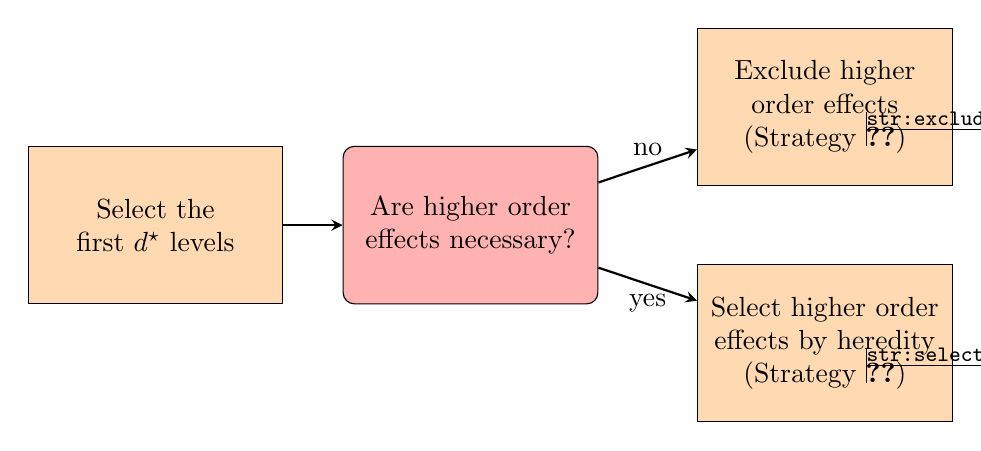
\begin{tikzpicture}[node distance = 2cm]
\node (pro1) [process] {Select the first $d^\star$ levels};
\node (dec2) [startstop, right of=pro1, xshift=2cm] {Are higher order effects necessary? };
\node (pro4) [process, right of=dec2, xshift = 2.5cm, yshift = -1.5cm] {Select higher order effects by heredity (Strategy \ref{str:select-by-heredity})};
\node (pro5) [process, right of=dec2, xshift = 2.5cm,  yshift = 1.5cm] {Exclude higher order effects (Strategy \ref{str:exclude-all})};

\draw [arrow] (pro1) -- (dec2);
\draw [arrow] (dec2) -- node[anchor=north] {yes} (pro4);
\draw [arrow] (dec2) -- node[anchor=south] {no} (pro5);

\end{tikzpicture}
\caption{General strategy for factorial  screening}
\label{fig:general-strategy}
\end{figure}


When using Algorithm \ref{alg:forward-ms}, we might believe that perfect selection is more plausible in the initial levels (say the main effects plus two way interactions). However, it can be problematic in the higher order interactions if the higher order interactions are too small in magnitude or the parameter $\alpha_d$ at a particular layer is not well-tuned. Therefore, it is reasonable to start from the situation where we are only assured perfect selection for the first several levels:
\begin{condition}\label{cond:under-selection}
The selected working model is correct up to the level $d^\star \le D^\star$ with  probability tending to 1:
\begin{align*}
    \Prob{\hat{\bbM}_1 = \bbM^\star_1, \dots, \hat{\bbM}_{d^\star} = \bbM^\star_{d^\star}} \to 1. 
\end{align*}
\end{condition}

Condition \ref{cond:under-selection} does not impose any restriction on the selection results beyond level $d^\star$. For example, in practice we can set $d^\star = 2$ if we do not have confidence in the selection results beyond main effects and second-order interactions. This motivates the first strategy without perfect model selection:

\begin{strategy}[Exclude higher order interactions]\label{str:exclude-all}
 In Algorithm \ref{alg:forward-ms}, set $\alpha_d = \infty,d\ge d^\star + 1$ so that no effects beyond level $d^\star$ will be selected and $\hat{\bbM} = \cup_{d=1}^{d^\star}\hat{\bbM}_{d}$. 
\end{strategy}

Strategy \ref{str:exclude-all} leads to under-selection: $\hat{\bbM}\subset{\bbM}^\star$. In this case, unbiasedness usually fails for estimating general linear combination of average potential outcomes:
\begin{align}
    \bsf^\top \overline{Y} =& \bsf^\top G(\cdot,\bbM^\star)\tau(\bbM^\star)\notag \\
    =&  \sum_{d=1}^{d^\star}\bsf^\top G(\cdot,\bbM^\star_d)\tau(\bbM^\star_d) + \sum_{d=d^\star+1}^{D^\star} \bsf^\top G(\cdot,\bbM^\star_d)\tau(\bbM^\star_d). \label{eqn:decomposition}
\end{align}
Because the selected working model might deviate from the truth beyond level $d^\star$, we do not have a consistent estimation for the second part of \eqref{eqn:decomposition}. Therefore, we will need to focus on  coefficient vectors $\bsf$ that satisfy the some orthogonality conditions as introduced in Theorem \ref{thm:strategy-I} below:
\begin{theorem}[Guarantee for Strategy \ref{str:exclude-all}]\label{thm:strategy-I}
Assume Conditions \ref{cond:nondegenerate-corr} and \ref{cond:under-selection}. Also assume $\bsf$ satisfies the following orthogonality condition: 
\begin{align}\label{eqn:orthogonality}
    G(\cdot, \bbM_d^{\star})^\top\bsf = 0, ~d^\star +1 \le d \le D^\star.
\end{align}
Let $ {\bsf}[\bbM^\star_{1:d^\star}]$ be given by \eqref{eqn:bsf-M} with $\bbM^\star_{1:d^\star} = \cup_{d=1}^{d^\star}\bbM^\star_d$. If 
\begin{align*}
    \frac{  \max_{i\in[N],\bz\in[Q]}|Y_i(\bz)-\overline{Y}(\bz)|}{\sqrt{  \min_{\bz\in[Q]} S(\bz,\bz)}\cdot \sqrt{N_0}}\cdot  \frac{\|{\bsf}[\bbM^\star_{1:d^\star}]\|_\infty}{\|{\bsf}[\bbM^\star_{1:d^\star}]\|_2} \longrightarrow 0,
\end{align*}
then 
\begin{align*}
    \frac{\hgamma[\hat{\bbM}]-\gamma}{v[\bbM^\star_{1:d^\star}]} \rightsquigarrow \cN(0,1).
\end{align*}

\end{theorem}

\eqref{eqn:orthogonality} states that the coefficient vector $\bsf$ should be orthogonal to the higher order contrasts, which makes sense because the under selection procedure cannot provide  screening guarantee for high order interactions. One straightforward example satisfying  \eqref{eqn:orthogonality} is linear combination of lower-order contrasts, given by
\begin{align*}
\bsf = G(,\cup_{d=1}^{d^\star}\bbM^\star_d) \boldsymbol{b}.
\end{align*}
For any $d_0\ge d^\star + 1$, we can calculate
\begin{align*}
    G(\cdot, \bbM_{d_0}^{\star})^\top\bsf = G(\cdot, \bbM_{d_0}^{\star})^\top G(,\cup_{d=1}^{d^\star}\bbM^\star_d) \boldsymbol{b} = 0,
\end{align*}
which holds due to the orthogonality between low order and higher order contrasts. 




On the other hand, in certain scenarios people do care about higher order interactions, for which the screening procedure might not  work perfectly. To this end, we propose to select the effects by hierarchy which takes higher order effects into consideration and guarantees high interpretability over the selected model. 


\begin{strategy}[Select higher order interactions by heredity]\label{str:select-by-heredity}
In Algorithm \ref{alg:forward-ms}, set $\alpha_d = 0,d\ge d^\star+1$ and apply a heredity principle (either weak or strong, depending on people's knowledge on the structure of the effects). Then the high order effects beyond level $ d^\star$ are selected merely by heredity principle and 
$$
\hat{\bbM} = \cup_{d=1}^{D}\hat{\bbM}_{d}; ~\hat{\bbM}_{d} = \texttt{\em H}^{(d-d^\star)}(\hat{\bbM}_{d^\star}), d\ge d^\star+1.
$$
Here $\texttt{\em H}^{(d-d^\star)}$ is the $(d-d^\star)$-order composition of $\texttt{\em H}$, meaning applying $\texttt{\em H}$ for $(d-d^\star)$ times.
\end{strategy}


We have the following results for Strategy \ref{str:select-by-heredity}:
\begin{theorem}[Guarantee for Strategy \ref{str:select-by-heredity} ]\label{thm:strategy-II}
Assume Conditions \ref{cond:nondegenerate-corr}, \ref{cond:heredity} and \ref{cond:under-selection}. Let 
\begin{align*}
    \bbM^{\star\star} = \bigcup_{d=1}^D \bbM^{\star\star}_d,
\end{align*}
where
\begin{align*}
    \bbM^{\star\star}_d = \left\{
    \begin{array}{cc}
        \bbM^{\star}_d, & d\le d^\star; \\
        \texttt{\em H}^{(d-d^\star)}(\bbM^{\star}_{d^\star}), & d^\star+1\le d\le D.
    \end{array}
    \right.
\end{align*}
Then 
\begin{align*}
    \bbM^\star \subset \bbM^{\star\star},~ \Prob{\hat{\bbM} = \bbM^{\star\star}} \to 1.
\end{align*}
Let $ {\bsf}[\bbM^{\star\star}]$ be given by \eqref{eqn:bsf-M} with $\bbM = \bbM^{\star\star} $. If 
\begin{align*}
    \frac{\max_{i\in[N],\bz\in[Q]}|Y_i(\bz)-\overline{Y}(\bz)|}{\sqrt{ \min_{\bz\in[Q]} S(\bz,\bz)}\cdot \sqrt{N_0}}\cdot  \frac{\|{\bsf}[\bbM^{\star\star}]\|_\infty}{\|{\bsf}[\bbM^{\star\star}]\|_2} \longrightarrow 0,
\end{align*}
then 
\begin{align*}
    \frac{\hgamma[\hat{\bbM}]-\gamma}{v[\bbM^{\star\star}]} \rightsquigarrow \cN(0,1).
\end{align*}



\end{theorem}


Strategy \ref{str:select-by-heredity} is an over-selection procedure because $\bbM^\star\subset\hat{\bbM}$ with high probability. For one thing, Strategy \ref{str:select-by-heredity} can guarantee the inclusion of the true model. For another thing, Strategy \ref{str:select-by-heredity} preserves the heredity structure in the effects so that the selected working model has high interpretability in practice.  


When analyzing Strategy \ref{str:exclude-all} and \ref{str:select-by-heredity},  the selected working model recovers a fixed model with high probability. Both strategies have advantages and disadvantages. Under-selection reflects bias-variance trade-off: it can induce more bias for certain target parameters, but the constructed estimator typically enjoys smaller variance. Over-selection typically reduces bias for estimation but suffers from loss of efficiency compared with perfect screening because one might include too many redundant terms into the selected model. In general, if higher order interactions are not crucial for study, Strategy \ref{str:select-by-heredity} should be applied. If high order interactions are of interest and hard to select, one could pursue Strategy \ref{str:exclude-all} as a practically useful and interpretable solution.

\section{Simulation}

\section{More discussions}

\subsection{Discussion of several  screening methods in finite population factorial experiments}
\begin{itemize}
\item Bonferroni correction:

\item LASSO: {\color{red} soft thresholding!}
\begin{align*}
    \min_{\tau \in \mathbb{R}^H}\sum_{i= 1}^N (y_i - f_i^\top \tau) + \lambda \|\tau\|_1,
\end{align*}

\item AIC: {\color{red} hard thresholding!}
\begin{align*}
    \min_{\tau \in \mathbb{R}^H,\bbM\subset [K]}\sum_{i= 1}^N (y_i - f_i^\top \tau_{\bbM}) + \lambda |\bbM|,
\end{align*}

\item BIC: {\color{red} hard thresholding!}
\begin{align*}
    \min_{\tau \in \mathbb{R}^H, \bbM\subset [K]}\sum_{i= 1}^N (y_i - f_{i,\bbM}^\top \tau_{\bbM}) + \lambda |\bbM| \log(N),
\end{align*}
\end{itemize}


\subsection{Discussion: more general centering values}

\subsubsection{Unsaturated weighted least square: a closed form expression}

In this section we first derive the closed form expression for unsaturated WLS estimation, then verify the nice targeting property we mentioned in the previous section. 

First we need to introduce a transformation matrix $\bP_{\Delta\delta_{[K]}}$, with columns and rows indexed by subsets $\{\cK\subset [K]\}$ of the $K$ factors. Generally it is used to reveal the relationship between designs with different configurations of centering factors $\delta_{[K]}$ and $\delta'_{[K]} = \delta_{[K]}+\Delta\delta_{[K]}$. The transformation is actually linear:
\begin{align}
    \left(f_{\delta'_{[K]}}(z^*_\cK)\right)_{\cK\subset [K]} = \left(f_{\delta_{[K]}}(z^*_\cK)\right)_{\cK\subset [K]} \bP_{\Delta\delta_{[K]}}.
\end{align}

The closed form of $\bP_{\Delta\delta_{[K]}}$ is easy to derive.  Note that for all $\cK'\subset [K]$, we have 
\begin{align}
    f_{\delta'_{[K]}}(z^*_{\cK'}) = \sum_{\cK\subset \cK'}f_{\delta_{[K]}}(z^*_{\cK}) \prod_{k\in \cK'\backslash \cK}(\Delta\delta)_k, \notag
\end{align}
which implies the element of $\bP_{\Delta\delta_{[K]}}$ indexed by $(\cK, \cK')$ is given by
\begin{align}\label{eqn:Pmatrix}
\bP_{\Delta\delta_{[K]}}(\cK,\cK')=\left\{
\begin{array}{ccc}
    \prod_{k\in \cK'\backslash \cK}(\Delta\delta)_k &, & \cK\subset\cK', \\
     0 &, & \cK\subsetneq \cK'. 
\end{array}
\right.
\end{align}

Define $\bQ_{\Delta\delta_{[K]}} = \bP_{\Delta\delta_{[K]}}^{-1}$ to be the inverse. Note that $\bQ_{\Delta\delta_{[K]}}$ is simply taking out a $\Delta\delta_{[K]}$ vector from a group of centering factors, so by symmetry we have 
\begin{align}\label{eqn:Qmatrix}
    \bQ_{\Delta\delta_{[K]}}(\cK,\cK') = \left\{
\begin{array}{ccc}
    (-1)^{|\cK'|-|\cK|}\prod_{k\in \cK'\backslash \cK}(\Delta\delta)_k &, & \cK\subset\cK', \\
     0 &, & \cK\subsetneq \cK'. 
\end{array}
\right.
\end{align}

We shall give an example of the above matrix in the three-factor case, which appears (incompletely) in the appendix of \cite{zhao2021regression}. Let $A'=A-\delta_A$, $B'=B-\delta_B$, $C'=C-\delta_C$. 
\begin{align*}
    \begin{pmatrix}
    1\\
    A\\
    B\\
    C\\
    AB\\
    AC\\
    BC\\
    ABC
    \end{pmatrix} = \bP_{\Delta\delta_{[K]}}^\top 
    \begin{pmatrix}
    1\\
    A'\\
    B'\\
    C'\\
    A'B'\\
    A'C'\\
    B'C'\\
    A'B'C'
    \end{pmatrix}=
    \begin{pmatrix}
    1        & 0 & 0 & 0 & 0 & 0 & 0 & 0 \\
    \delta_A & 1 & 0 & 0 & 0 & 0 & 0 & 0 \\
    \delta_B & 0 & 1 & 0 & 0 & 0 & 0 & 0 \\
    \delta_C & 0 & 0 & 1 & 0 & 0 & 0 & 0 \\
    \delta_A\delta_B & \delta_B & \delta_A & 0 & 1 & 0 & 0 & 0\\ 
    \delta_A\delta_C & \delta_C & 0 & \delta_A & 0 & 1 & 0 & 0\\ 
    \delta_B\delta_C & 0 & \delta_C & \delta_B & 0 & 0 & 1 & 0\\ 
    \delta_A\delta_B\delta_C & \delta_B\delta_C & \delta_A\delta_C & \delta_A\delta_B & \delta_C & \delta_B & \delta_A & 1\\
    \end{pmatrix}
    \begin{pmatrix}
    1\\
    A'\\
    B'\\
    C'\\
    A'B'\\
    A'C'\\
    B'C'\\
    A'B'C'
    \end{pmatrix}.
\end{align*}

The following theorem shows that $\bP_{\Delta\delta_{[K]}}$ and $\bQ_{\Delta\delta_{[K]}}$ totally determines the structure of $\bD_h$.


\begin{theorem}\label{thm:closeD}
Consider weighted least squares with centering factors $\delta_{[K]}$ and weights proportional to size of  each stratum. Let $\Delta\delta_{[K]} = \delta_{[K]}-(1/2)_{k=1}^K$. The unsaturated regression  on up to all $m$-level main/interactions terms has coefficient vector:
\begin{align}\label{eqn:wls-res}
    (\tilde{\tau}_{\cK})_{\{|\cK|\le m\}} = ({\tau}_{\cK})_{\{|\cK|\le m\}} + \bD_h\cdot({\tau}_{\cK})_{\{|\cK|> m\}},
\end{align}
where $\bD_h$ is given by 
\begin{align*}
    \bD_h = \bP_{\Delta\delta_{[K]}}\left(\{\cK\subset [m]\}, \{\cK\subset [m]\}\right) \cdot \bQ_{\Delta\delta_{[K]}}\left(\{\cK\subset [m]\}, \{\cK\subset [K] \backslash[m]\}\right).
\end{align*}
\end{theorem}




\begin{corollary}\label{cor:closeD}
The matrix $\bD$ has a closed form expression:
\begin{enumerate}
    \item For $\cK\subsetneq \cK'$,
    \begin{align}
    \bD_h(\cK, \cK') = 0.
    \end{align}
     
    \item For $\cK\subset \cK'$, let $|\cK|=k$, $|\cK'|=k'$, with $k\le m <k'$,
    \begin{align}
    \bD_h(\cK, \cK') = \sum_{l=0}^{m-k} (-1)^{k'-k+1-l} \begin{pmatrix}
    k'-k+1 \\
    l
    \end{pmatrix}
    \prod_{t\in \cK'\backslash \cK}\left(\delta_t-\frac{1}{2}\right).
    \end{align}
\end{enumerate}

\end{corollary}

\begin{proof}
This result can be derived through careful calculation based on the definition of $\bP$ and $\bQ$ from \eqref{eqn:Pmatrix} and \eqref{eqn:Qmatrix} along with Theorem \ref{thm:closeD} thus omitted here. 
\end{proof}


\subsubsection{A sufficient condition for sign consistency in population WLS regression}

\begin{definition}[Active interaction number]\label{def:sparsity}
For every $z_k$ of the $K$ factors, there are $s_k$ factors that have nonzero interaction with $z_k$, where $s_k\in [K-1]$ is a nonnegative integer associated with $K$. We call $s_k$ the active interaction number of factor $z_k$. The maximal active interaction number is subsequently defined as $s_K = \max_{k\in [K]} s_k$.
\end{definition}

This definition is mainly devoted to finer technical purposes in Theorem \ref{thm:suffcond}. 

\begin{theorem}\label{thm:suffcond}
Assume we run weighted least square under the setting depicted in  Theorem \ref{thm:closeD}. Define the maximal decaying rate $c_K=\max_{l\in[K]} c_l$. Recall the predefined maximal active interaction number $s_K$ from Definition \ref{def:sparsity}. If we have 
\begin{align}
s_Kc_K\max_{k=1,\dots,K} |\delta_k-1/2|<\ln 2, \label{cond:sufficient}
\end{align}
then the unsaturated regression coefficients
$(\tilde{\tau}_{\cK})_{\{|\cK|\le m\}}$ and the corresponding saturated regression coefficients  $({\tau}_{\cK})_{\{|\cK|\le m\}}$ from \eqref{eqn:wls-res} have same signs on every term.

\end{theorem}

Condition \eqref{cond:sufficient} unifies the property of factorial effects and the information of the design pattern(the centering factors $\delta_{[K]}$). The product of $s_K$ and $c_K$ demonstrates a trade-off between the active interaction number and the hierarchy structure. Sparser interactions require slower decaying rate and vice versa. Besides, the product of $s_Kc_K$ and $\max_{k=1,\dots,K} |\delta_k-1/2|$ shows that if $\delta_k$ lies more close to $1/2$, less restriction are needed on the effect structure. This aligns with the result in \cite{zhao2021regression}: when $\delta_k=1/2$ holds for all $k=1,\dots, K$,  $\bD_h=\boldsymbol{0}$, so that forward selection always works. 


\section{Conclusion}

\bibliographystyle{apalike}
\bibliography{ref.bib}

\appendix



\section{General results on consistency of forward screening}

We are now ready to show the guarantee for our procedure. Our presentation starts from a theorem (Theorem \ref{thm:ms-consistency}) quantifying the performance of the forward procedure \eqref{eqn:track-model} under general assumptions on the S-step and P-step. Then we derive a corollary (Theorem \ref{thm:marginal-t}) by specifying the S-step as Bonferroni corrected marginal t tests and the P-step as screening based on heredity.  The high level of the proof proceeds through mathematical induction:
\begin{enumerate}
    \item (Base case) Show that forward screening selects the correct main effects with probability tending to one.
    
    \item (Induction step) Show that if we correctly screen the effects up to $k$-way interactions (main effects if $k=1$), then we are able to correctly detect the non-nulls among all $(k+1)$-way interactions. 
\end{enumerate}

\commenting{
Recall that the validity of a test requires that given the null is true, the probability of rejection should be less than the pre-specified significance level. The consistency of a test, on the other hand, requires that when the alternative is true, we have probability tending to 1 to reject the null.  Following the tradition in the realm of  screening \citep{wasserman2009high}, we introduce the following definitions:
\begin{definition}[Terminologies for  screening]
The following terminologies are wrapped up for the discussion of  screening:
\begin{itemize}
    \item Type I error:  commit a false positive. Because the selected positives are contained in $\hat{\bbM}$, this translates into $\hat{\bbM}\cap\bbM^{\star c}\neq \varnothing$. 
    \item Type II error:  commit a false negative. Because the selected negatives are contained in $\hat{\bbM}$, this translates into $\hat{\bbM}^c\cap\bbM^{\star}\neq \varnothing$. 
\end{itemize}
\end{definition}

Clearly size measures the ability of under-selection; because zero $q(\hat{\bbM})$ means $\hat{\bbM}\subset \bbM^\star$. Power measures the ability of over-selection, because a power of 1 means $\bbM^\star\subset\hat{\bbM}$. We have the following graph to visualize the idea:



%\tikzset{every picture/.style={line width=0.75pt}} %set default line width to 0.75pt        
\begin{figure}[th]
\centering


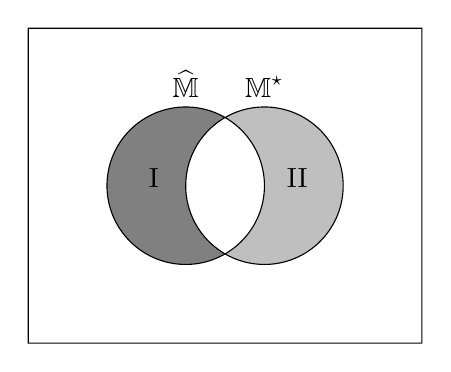
\begin{tikzpicture}[fill]
% left hand
\scope
\clip (-2,-2) rectangle (2,2)
      (1,0) circle (1);
\fill[gray] (0,0) circle (1);
\endscope
% right hand
\scope
\clip (-2,-2) rectangle (2,2)
      (0,0) circle (1);
\fill[lightgray] (1,0) circle (1);
\endscope
% outline
\draw (0,0) circle (1) (0,1)  node [text=black,above] {$\displaystyle \hat{{\bbM}}$}
      (1,0) circle (1) (1,1)  node [text=black,above] {$\displaystyle {\bbM}^{\star}$}
      (-2,-2) rectangle (3,2);
      
% Text Node
\draw (1.25,0.25) node [anchor=north west][inner sep=0.75pt]   [align=left] {II};
% Text Node
\draw (-0.5,0.25) node [anchor=north west][inner sep=0.75pt]   [align=left] {I};
      
      
      
\end{tikzpicture}
\label{fig:error-visual}
\caption{Visualization of the two types of errors} screening

\end{figure}
}


In order to achieve satisfactory screening results, some regularization conditions need to be imposed to characterize a ``good" layer-wise S-step, and the P-step should ensure that the procedure progress in a way that is compatible with the structure of the true factorial effects.  In light of this, we use ${\bbM}^\star_{d,+}$ to denote the pruned set of effects on the $d$-th layer based on the true model $\bbM_{d-1}^\star$ on the previous layer; that is,
\begin{align*}
    {\bbM}^\star_{d,+} = \texttt{H}({\bbM}^\star_{d-1}).
\end{align*}
These discussions motivate the following assumption on the layer-wise selection procedure $\hat{\texttt{S}}(\cdot)$:
\begin{assumption}[Validity and consistency of the selection operator]\label{asp:valid-consistent}
We denote 
\begin{align*}
    \tilde{\bbM}_{d} = \hat{\text{\em \texttt{S}}}(\bbM^{\star}_{d,+};\{Y_i,Z_i\}^N_{i=1}),
\end{align*}
where $\bbM^{\star}_{d,+} = \text{\em \texttt{H}}(\bbM^{\star}_{d-1})$ is defined as above. Let $\{\alpha_d\}_{d=1}^D$ be a sequence of significance levels in $(0,1)$. We assume that the following \emph{validity} and \emph{consistency} property hold for $\text{\em \texttt{S}}_N(\cdot)$: for $d = 1,\cdots, D$, we have
\begin{align}
    \text{Validity:}&~\lim\sup_{N\to\infty}\bbP\lt\{\tilde{\bbM}_{d}\cap\bbM^{\star c}_d\neq \varnothing\rt\}\le \alpha_d,  \label{eqn:validity}\\
    \text{Consistency:}&~\lim\sup_{N\to\infty}\bbP\lt\{\tilde{\bbM}_{d}^c\cap\bbM^{\star}_d\neq \varnothing\rt\} = 0.  \label{eqn:consistency}
\end{align}
\end{assumption}


This assumption can be verified for many  screening procedures. In Theorem \ref{thm:marginal-t} we will show it holds for the layer-wise Bonferroni corrected marginal testing procedure in Algorithm \ref{alg:forward-ms}. Moreover, in the high dimensional super population study, a combination of data splitting, adaptation of $\ell_1$ regularization and marginal t tests can also fulfill such a requirement \citep{wasserman2009high}.




Besides, we assume the $\texttt{H}(\cdot)$ operator respects the structure of the nonzero factorial effects:
\begin{assumption}[H-heredity]\label{asp:H-heredity}
For $d=1,\cdots,D-1$, it holds
\begin{align*}
\bbM^\star_{d+1}\subset\texttt{\em P}(\bbM^\star_{d}).
\end{align*}
\end{assumption}

One special case of $\texttt{H}(\cdot)$ operator satisfying Assumption \ref{asp:H-heredity} is naively adding all the the higher order interactions regardless of the lower-order screening results. Besides, if we have evidence that the effects have particular hierarchical structure, applying the corresponding heredity principle such as \eqref{eqn:weak-heredity} or \eqref{eqn:strong-heredity} can improve screening accuracy as well as interpretability of the screening results.
\begin{theorem}[Screening consistency]\label{thm:ms-consistency}
Assume $\bbM^\star\neq\varnothing$. Assume Assumption \ref{asp:valid-consistent} and \ref{asp:H-heredity}.  Then the forward screening procedure \eqref{eqn:track-model} has the following properties:

\begin{enumerate}[label = (\roman*)]
    \item {\em Type I error control.} Forward screening controls the Type I error rate, in the sense that 
    \begin{align}
        \underset{N\to\infty}{\lim\sup}~\bbP\left(\hat{\bbM}_d\cap{\bbM_d^\star}^c\neq\varnothing \text{ for some } d\in [D]\right)\le \alpha = \sum_{d=1}^D \alpha_d.
    \end{align}
    \item {\em  Screening consistency.} Further assume $\alpha=\alpha_N\to0$. The forward procedure consistently selects all the nonzero effects up to $D$ levels with probability tending to 1: 
    \begin{align}
        \underset{N \to \infty}{\lim\sup}~\bbP\left(\hat{\bbM}_d = \bbM_d^\star \text{ for all }d\in[D]\right)=1.
    \end{align}
\end{enumerate}
\end{theorem}


Theorem \ref{thm:ms-consistency} consists of two parts. First, one can control the type I error rate, which is defined as the probability of over-selects at least one zero effect. The definition is introduced and elaborated detailedly in \cite{wasserman2009high} for model selection. Second, if the tuning parameter $\alpha = \sum_{d=1}^D\alpha_d$ vanish asymptotically, one can actually achieve perfect screening up to $D$ levels of effects.  To apply Theorem \ref{thm:ms-consistency} to specific procedures, the key step is to verify Assumption \ref{asp:valid-consistent} and justify Assumption \ref{asp:H-heredity}, which we will do for Bonferroni corrected marginal t tests as an example in the next section.

Moreover, the scaling of $\alpha_N$ plays an important role in theoretical discussion. To achieve perfect selection, we hope $\alpha_N$ decays as fast as possible; ideally if $\alpha_N$ equals zero then we do not commit any type I error (or equivalently, we will never select redundant effects). However, for many data-dependent selection procedure $\alpha$ can only decay at certain rates, because a fast decaying $\alpha$ means higher possibility of rejection, thus can lead to strict under-selection. Therefore, in the tuning process, $\alpha_d$ should be scaled properly if one wants to pursue perfect selection. Nevertheless, even if the tuning is hard and perfect model selection can not be achieved, we still have many strategies to exploit the advantage of the forward screening procedure. We will have more discussions in later sections.




\section{Technical proofs}
\subsection{Preliminaries: some important probabilistic results in randomized experiments}

Consider an estimator of the form
\begin{align*}
    \hgamma = Q^{-1}\sum_{\bz\in\cT} w(\bz)\hat{Y}(\bz),
\end{align*}
with variance estimation
\begin{align*}
    \hat{v}^2_R = Q^{-2}\sum_{\bz\in\cT} w(\bz)^2 \hat{S}(\bz,\bz).
\end{align*}

We have the following variance estimation results and Berry-Esseen bounds:

\begin{lemma}[Variance concentration and Berry-Esseen bounds in finite population]\label{lem:BE-finite-pop}
Denote $\gamma = \bbE\{\hgamma\}$, $v^2 = \operatorname{Var}(\hgamma)$ and $v^2_R = \bbE\{\hat{v}^2_R\}$.
Suppose the following conditions hold: 
\begin{itemize}
    \item  Nondegenerate variance. There exists a $\sigma_w > 0$, such that
    \begin{align}\label{eqn:nondegenerate-var}
        Q^{-2}\sum_{\bz=1}^Q w(\bz)^2 N_{\bz}^{-1} S(\bz,\bz) \le \sigma_w^2 v^2.
    \end{align}
    
    \item Bounded fourth moments. There exists a $ \delta > 0$ such that
    \begin{align}\label{eqn:bounded-moments}
    \max_{\bz\in[Q]}\frac{1}{N}\sum_{i=1}^N \{Y_i(\bz) - \overline{Y}(\bz)\}^4 \le \Delta^4.
    \end{align}
\end{itemize}


\begin{enumerate}
    \item The variance estimator is robust for the true variance:
    $v_R \ge v$. Besides, the following tail bound holds:
    \begin{align}\label{eqn:tail-vhatR}
        \bbP\lt\{N |\hat{v}_R-v_R | > t\rt\} 
        \le \frac{C\overline{c}^3\underline{c}^{-4} \|w\|_\infty^2 \Delta^4 }{QN_0}\cdot \frac{1}{t^2}.
    \end{align}

    \item We have a Berry-Esseen bound with the true variance:
    \begin{align}\label{eqn:uniform-design-be}
       \sup_{t\in\bbR}\lt|\Prob{\frac{\hgamma-\gamma}{v} \le t} - \Phi(t)\rt|  \le  2C\sigma_w   \frac{\underline{c}^{-1}  \|w\|_{\infty}   \max_{i\in[N],\bz\in[Q]}|Y_i(\bz)-\overline{Y}(\bz)|}{\|w\|_2\sqrt{\overline{c}^{-1} \min_{\bz\in[Q]} S(\bz,\bz)}\cdot \sqrt{ N_0}} .
    \end{align}
    
    \item We have a Berry-Esseen bound with the estimated variance: for any $\epsilon_N \in (0, 1/2]$,
    \begin{align*}
        \sup_{t\in\bbR}\lt|\bbP\lt\{\frac{\hgamma - \gamma}{\hat{v}_R} \le t\rt\} - \Phi\lt(\frac{v_R}{v}t\rt)\rt| &\le
        \epsilon_N +  \frac{C\overline{c}^3\underline{c}^{-4} \|w\|_\infty^2 \Delta^4 }{QN_0}\cdot \frac{1}{(Nv^2\epsilon_N)^2} \\
        &+ 2C\sigma_w   \frac{\underline{c}^{-1}  \|w\|_{\infty}   \max_{i\in[N],\bz\in[Q]}|Y_i(\bz)-\overline{Y}(\bz)|}{\|w\|_2\sqrt{\overline{c}^{-1} \min_{\bz\in[Q]} S(\bz,\bz)}\cdot \sqrt{N_0}}.
    \end{align*}
\end{enumerate}

\end{lemma}

\showproof{\showproofFlag}{
\begin{proof}[Proof of Lemma \ref{lem:BE-finite-pop}]
\begin{enumerate}
    \item {\color{red} BE-PCLT Corollary 2}.

    \item {\color{red} BE-PCLT Theorem 8}.
    
    \item Proof of the third part. First we show a useful result: for $|a|\le 1/2$ and any $b\in\bbR$, 
    \begin{align}\label{form:Phi-bD}
        \sup_{t\in\bbR}|\Phi\{(1+a)t + b\} - \Phi\{t\}| \le |a| + |b|.
    \end{align}
    This can be proved by a simple step of intermediate value theorem: for any $t\in\bbR$,
    \begin{align*}
        &|\Phi\{(1+a)t + b\} - \Phi\{t\}| \\
        =& |\phi(\xi_{t,(1+a)t})\cdot (at + b)|\\
        =& |\phi(\xi_{t,(1+a)t})\cdot at| + |\phi(\xi_{t,(1+a)t})\cdot b|\\
        =& |a| \cdot |\phi(\xi_{t,(1+a)t})\cdot t|\cdot \ind{|t|\le 1} + |a| \cdot |\phi(\xi_{t,(1+a)t})\cdot t|\cdot \ind{|t| > 1} + |\phi(\xi_{t,(1+a)t})\cdot b|\\
        \le& \frac{1}{\sqrt{2\pi}}|a|\cdot \ind{|t|\le 1} + \frac{1}{\sqrt{2\pi}} |a| |t|\cdot\exp(-t^2/8)\cdot\ind{|t| > 1} +  {\frac{1}{\sqrt{2\pi}}}|b|\\
        \le& |a| + |b|.
    \end{align*}
    WLOG we consider $t\ge 0$ because $t<0$ can be handled similarly. For any $\epsilon_N > 0$, We have
    \begin{align*}
        \bbP\lt\{\frac{\hgamma - \gamma}{\hat{v}_R} \le t\rt\} &= \bbP\lt\{\frac{\hgamma - \gamma}{{v}} \le \frac{\hat{v}_R}{{v}}t\rt\}\\
        &= \bbP\lt\{\frac{\hgamma - \gamma}{{v}} \le \frac{\hat{v}_R}{{v}}t, \lt|\frac{\hat{v}_R - v_R}{v}\rt| \le \epsilon_N\rt\} + \bbP\lt\{\frac{\hgamma - \gamma}{{v}} \le \frac{\hat{v}_R}{{v}}t, \lt|\frac{\hat{v}_R - v_R}{v}\rt| > \epsilon_N\rt\}.
    \end{align*}
    Then we can show that
    \begin{align*}
        \bbP\lt\{\frac{\hgamma - \gamma}{\hat{v}_R} \le t\rt\} &\le 
        \bbP\lt\{\frac{\hgamma - \gamma}{{v}} \le \frac{\hat{v}_R}{{v}}t, \lt|\frac{\hat{v}_R - v_R}{v}\rt| \le \epsilon_N\rt\} + \bbP\lt\{ \lt|\frac{\hat{v}_R - v_R}{v}\rt| > \epsilon_N\rt\}\\
        &\le \bbP\lt\{\frac{\hgamma - \gamma}{{v}} \le \lt(\frac{{v}_R}{v} + \epsilon_N\rt)t\rt\} + \bbP\lt\{ \lt|\frac{\hat{v}_R - v_R}{v}\rt| > \epsilon_N\rt\}.
    \end{align*}
    
    For the first term, we have
    \begin{align*}
        &\sup_{t\ge 0}\lt|\bbP\lt\{\frac{\hgamma - \gamma}{{v}}   \le \lt(\frac{{v}_R}{v} + \epsilon_N\rt)t\rt\} - \Phi\lt\{\lt(\frac{{v}_R}{v} + \epsilon_N\rt)t \rt\}\rt| \\
        &\le 2C\sigma_w   \frac{\underline{c}^{-1}  \|w\|_{\infty}   \max_{i\in[N],\bz\in[Q]}|Y_i(\bz)-\overline{Y}(\bz)|}{\|w\|_2\sqrt{\overline{c}^{-1} \min_{\bz\in[Q]} S(\bz,\bz)}\cdot \sqrt{ N_0}}.
    \end{align*}
    For the second term, using the variance estimation results in Part 1 we have
    \begin{align*}
        \bbP\lt\{ \lt|\frac{\hat{v}_R - v_R}{v}\rt| \ge \epsilon_N\rt\} &\le  \bbP\lt\{ \lt|\frac{\hat{v}_R - v_R}{v}\rt|\cdot\lt|\frac{\hat{v}_R + v_R}{v}\rt| \ge \epsilon_N\rt\} \see{because $v_R$ is robust}\\
        & =  \bbP\lt\{ \lt|\frac{N\hat{v}^2_R - Nv^2_R}{Nv^2}\rt| \ge \epsilon_N\rt\}   \\
        & \le \frac{C\overline{c}^3\underline{c}^{-4} \|w\|_\infty^2 \Delta^4 }{QN_0}\cdot \frac{1}{(Nv^2\epsilon_N)^2}.
    \end{align*}
    Besides, by \eqref{form:Phi-bD}, when $\epsilon_N\le 1/2$, we also have
    \begin{align*}
        \sup_{t\in\bbR}\lt|\Phi\lt\{\lt(\frac{{v}_R}{v} + \epsilon_N \rt)t \rt\} - \Phi\lt(\frac{v_R}{v}t\rt)\rt| \le \frac{v\epsilon_N}{v_R} \le \epsilon_N. 
    \end{align*}
    Aggregating all the parts above, we can show that for any $t\ge 0$,
    \begin{align*}
        \bbP\lt\{\frac{\hgamma - \gamma}{\hat{v}_R} \le t\rt\} &\le \Phi\lt(\frac{v_R}{v}t\rt) + \epsilon_N +  \frac{C\overline{c}^3\underline{c}^{-4} \|w\|_\infty^2 \Delta^4 }{QN_0}\cdot \frac{1}{(Nv^2\epsilon_N)^2} \\
        &+ 2C\sigma_w   \frac{\underline{c}^{-1}  \|w\|_{\infty}   \max_{i\in[N],\bz\in[Q]}|Y_i(\bz)-\overline{Y}(\bz)|}{\|w\|_2\sqrt{\overline{c}^{-1} \min_{\bz\in[Q]} S(\bz,\bz)}\cdot \sqrt{N_0}}.
    \end{align*}
    
    On the other hand, we can show that
    \begin{align}
        \bbP\lt\{\frac{\hgamma - \gamma}{\hat{v}_R} \le t\rt\} &\ge 
        \bbP\lt\{\frac{\hgamma - \gamma}{{v}} \le \frac{\hat{v}_R}{{v}}t, \lt|\frac{\hat{v}_R - v_R}{v}\rt| \le \epsilon_N\rt\} \notag\\
        &\ge \bbP\lt\{\frac{\hgamma - \gamma}{{v}} \le \lt(\frac{{v}_R}{v} - \epsilon_N\rt)t\rt\} - \bbP\lt\{ \lt|\frac{\hat{v}_R - v_R}{v}\rt| \ge \epsilon_N\rt\}.\label{eqn:upper-bd}
    \end{align}
    By \eqref{form:Phi-bD}, when $\epsilon_N\le 1/2$, we also have
    \begin{align*}
        \sup_{t\in\bbR}\lt|\Phi\lt\{\lt(\frac{{v}_R}{v} - \epsilon_N\rt)t \rt\} - \Phi\lt(\frac{v_R}{v}t\rt)\rt| \le \epsilon_N. 
    \end{align*}
    So we can derive a lower bound analogous to \eqref{eqn:upper-bd}. Note that the results can be analogously generalized to $t\le 0$. Putting pieces together, we can show that for any $t\ge 0$,
    \begin{align*}
        \sup_{t\in\bbR}\lt|\bbP\lt\{\frac{\hgamma - \gamma}{\hat{v}_R} \le t\rt\} - \Phi\lt(\frac{v_R}{v}t\rt)\rt| &\le
        \epsilon_N +  \frac{C\overline{c}^3\underline{c}^{-4} \|w\|_\infty^2 \Delta^4 }{QN_0}\cdot \frac{1}{(Nv^2\epsilon_N)^2} \\
        &+ 2C\sigma_w   \frac{\underline{c}^{-1}  \|w\|_{\infty}   \max_{i\in[N],\bz\in[Q]}|Y_i(\bz)-\overline{Y}(\bz)|}{\|w\|_2\sqrt{\overline{c}^{-1} \min_{\bz\in[Q]} S(\bz,\bz)}\cdot \sqrt{ N_0}}.
    \end{align*}
\end{enumerate}


\end{proof}
}

The following corollary shows the studentized Berry-Esseen bounds in the special case where $w = (w(\bz))_{\bz\in[Q]}$ is a contrast vector for factorial effects. That is, $ w = g_\cK$ for some $\cK \in \bbK $. 

\begin{corollary}\label{cor:factorial-student-be}
Assume Condition \eqref{eqn:nondegenerate-var} and \eqref{eqn:bounded-moments} hold. Let $ w = g_\cK$ for some $\cK \in \bbK $. Then we have a Berry-Esseen bound with the estimated variance:
\begin{align*}
    \sup_{t\in\bbR}\lt|\bbP\lt\{\frac{\htau_\cK - \tau_\cK}{\hat{v}_R} \le t\rt\} - \Phi\lt(\frac{v_R}{v}t\rt)\rt| &\le
          2\lt(\frac{C\sigma_w^4\overline{c}^5\underline{c}^{-6}  \Delta^4 }{\{\min_{\bz\in\cT}S(\bz,\bz)\}^2}\rt)^{1/3}\cdot\frac{1}{(QN_0)^{1/3}} \\
        &+ 2C\sigma_w   \frac{\underline{c}^{-1}     \max_{i\in[N],\bz\in[Q]}|Y_i(\bz)-\overline{Y}(\bz)|}{ \sqrt{\overline{c}^{-1} \min_{\bz\in[Q]} S(\bz,\bz)}}\cdot\frac{1}{(QN_0)^{1/2}}.
\end{align*}
\end{corollary}

\showproof{\showproofFlag}{
\begin{proof}[Proof of Corollary \ref{cor:factorial-student-be}]
\textbf{Lower bound for $Nv^2$.} Note that
$\|w\|_2^2 = Q, \|w\|_\infty = 1$. 
Using Condition \eqref{eqn:nondegenerate-var}, we have
\begin{align*}
    Nv^2 &\ge N\sigma_w^{-2} Q^{-2}\sum_{\bz=1}^Q w(\bz)^2 N_{\bz}^{-1} S(\bz,\bz) \\
    &\ge (\underline{c}QN_0)\cdot\sigma_w^{-2} \overline{c}^{-1}Q^{-1}N_{0}^{-1} \min_{\bz\in\cT} S(\bz,\bz) \cdot (Q^{-1}\|w\|_2^2)\\
    &= \sigma_w^{-2}\underline{c}\overline{c}^{-1}\min_{\bz\in\cT}S(\bz,\bz).
\end{align*}

Therefore, the Berry-Esseen bound becomes
\begin{align*}
    \sup_{t\in\bbR}\lt|\bbP\lt\{\frac{\htau_\cK - \tau_\cK}{\hat{v}_R} \le t\rt\} - \Phi\lt(\frac{v_R}{v}t\rt)\rt| &\le
        \epsilon_N +  \frac{C\sigma_w^4\overline{c}^5\underline{c}^{-6}  \Delta^4 }{(QN_0)\{\min_{\bz\in\cT}S(\bz,\bz)\}^2}\cdot \frac{1}{\epsilon_N^2} \\
        &+ 2C\sigma_w   \frac{\underline{c}^{-1}     \max_{i\in[N],\bz\in[Q]}|Y_i(\bz)-\overline{Y}(\bz)|}{\sqrt{\overline{c}^{-1} \min_{\bz\in[Q]} S(\bz,\bz)}\cdot \sqrt{QN_0}}.
\end{align*}

\textbf{Optimize the summation of the first and second term.}
By taking derivative over $\epsilon_N $ on the upper bound and solving for the zero point, we know that when 
\begin{align*}
    \epsilon_N = \lt(\frac{2C\sigma_w^4\overline{c}^5\underline{c}^{-6}  \Delta^4 }{(QN_0)\{\min_{\bz\in\cT}S(\bz,\bz)\}^2}\rt)^{1/3},
\end{align*}
the upper bound is minimized and 
\begin{align*}
    \sup_{t\in\bbR}\lt|\bbP\lt\{\frac{\htau_\cK - \tau_\cK}{\hat{v}_R} \le t\rt\} - \Phi\lt(\frac{v_R}{v}t\rt)\rt| &\le
          2\lt(\frac{C\sigma_w^4\overline{c}^5\underline{c}^{-6}  \Delta^4 }{\{\min_{\bz\in\cT}S(\bz,\bz)\}^2}\rt)^{1/3}\cdot\frac{1}{(QN_0)^{1/3}} \\
        &+ 2C\sigma_w   \frac{\underline{c}^{-1}     \max_{i\in[N],\bz\in[Q]}|Y_i(\bz)-\overline{Y}(\bz)|}{ \sqrt{\overline{c}^{-1} \min_{\bz\in[Q]} S(\bz,\bz)}}\cdot\frac{1}{(QN_0)^{1/2}}.
\end{align*}
\end{proof}
}

Additionally, we have a Berry-Esseen bounds after screening the effects:

\begin{lemma}[Berry Esseen bound with  screening]\label{lem:tail-perfect-ms} Let 
\begin{align}\label{eqn:tw}
{\bsf}[\bbM] = Q^{-1}G(\cdot,\bbM)G(\cdot,\bbM)^\top\bsf.
\end{align}
Assume there exists $\sigma_w>0$ such that
\begin{align}\label{eqn:nondegenerate-var-tw}
    \sum_{\bz=1}^Q {\bsf}[\bbM](\bz)^2 N_{\bz}^{-1} S(\bz,\bz) \le \sigma_w^2 v^2(\bbM).
\end{align}
Then it holds
\begin{align}\label{eqn:tail-perfect-ms}
    &\sup_{t\in\bbR}\lt|\Prob{\frac{\hgamma[\hat{\bbM}]-\gamma[\bbM]}{v(\bbM)} \le t} - \Phi(t)\rt| \notag\\
    &\le 2\Prob{\hat{\bbM}\neq \bbM} +  2C\sigma_w   \frac{\underline{c}^{-1} \max_{i\in[N],\bz\in[Q]}|Y_i(\bz)-\overline{Y}(\bz)|}{\sqrt{\overline{c}^{-1} \min_{\bz\in[Q]} S(\bz,\bz)}\cdot \sqrt{N_0}}\cdot  \frac{\|{\bsf}[\bbM]\|_\infty}{\|{\bsf}[\bbM]\|_2} .
\end{align}
\end{lemma}


{
\begin{proof}[Proof of Lemma \ref{lem:tail-perfect-ms}]
With the selected working model we have
\begin{align*}
    &\sup_{t\in\bbR}\lt|\Prob{\frac{\hgamma[\hat{\bbM}]-\gamma[\bbM]}{v(\bbM)} \le t} - \Phi(t)\rt| \\
    = &\sup_{t\in\bbR}\lt|\Prob{\frac{\hgamma[\hat{\bbM}]-\gamma[\bbM]}{v(\bbM)} \le t, \hat{\bbM} = \bbM} - \Phi(t) + \Prob{\frac{\hgamma[\hat{\bbM}]-\gamma[\bbM]}{v(\bbM)} \le t, \hat{\bbM} \neq \bbM} \rt|\\
    \le &\sup_{t\in\bbR}\lt|\Prob{\frac{\hgamma[\hat{\bbM}]-\gamma[\bbM]}{v(\bbM)} \le t, \hat{\bbM} = \bbM} - \Phi(t)\rt| +  \Prob{\frac{\hgamma[\hat{\bbM}]-\gamma[\bbM]}{v(\bbM)} \le t, \hat{\bbM} \neq \bbM}  \\
    = &\sup_{t\in\bbR}\lt|\Prob{\frac{\hgamma[{\bbM}]-\gamma[\bbM]}{v(\bbM)} \le t, \hat{\bbM} = \bbM} - \Phi(t)\rt| +  \Prob{\frac{\hgamma[\hat{\bbM}]-\gamma[\bbM]}{v(\bbM)} \le t, \hat{\bbM} \neq \bbM}  \\
    \le & \sup_{t\in\bbR}\lt|\Prob{\frac{\hgamma[{\bbM}]-\gamma[\bbM]}{v(\bbM)} \le t} - \Phi(t)\rt| +  2\Prob{ \hat{\bbM} \neq \bbM}.
\end{align*}

Now we have 
\begin{align*}
    \hgamma(\bbM) &= \bsf^\top G(\cdot, \bbM) \htau(\bbM) \\
    & =  \bsf^\top G(\cdot, \bbM) G(\cdot, \bbM)^\top \hY \\
    & = {\bsf}[\bbM]^\top \hY.
\end{align*}


By \inlinemod{red}{Corollary 2 of BE-PCLT},  we have a Berry-Esseen bound with the true variance:
\begin{align*}
    \sup_{t\in\bbR}\lt|\Prob{\frac{\hgamma( {\bbM})-\gamma[\bbM]}{v} \le t} - \Phi(t)\rt| 
    \le  2C\sigma_w   \frac{\|{\bsf}[\bbM]\|_\infty\underline{c}^{-1} \max_{i\in[N],\bz\in[Q]}|Y_i(\bz)-\overline{Y}(\bz)|}{\|{\bsf}[\bbM] \|_2\sqrt{\overline{c}^{-1} \min_{\bz\in[Q]} S(\bz,\bz)}\cdot \sqrt{ N_0}}.  
\end{align*}
    
\end{proof}
}



\subsection{Proof of Theorem \ref{thm:ms-consistency}}
{
\begin{proof}[Proof of Theorem \ref{thm:ms-consistency}]
\textbf{Induction proof of a basic fact.} According to the orthogonality of designs, the signs for all terms in the studied unsaturated population regressions are consistent with those of saturated regressions, which saves the effort of differentiating true models for partial and full regression. By induction we hope to prove the following fact under the given assumptions:


\begin{displayquote}
For all $D_0\le D$, we have 
\begin{align}\label{eqn:zerofn-general}
\lt|\bbP\lt(\hat{\bbM}_d\subset\bbM^\star_d, d=1,\cdots,D_0\rt)-\bbP\lt(\hat{\bbM}_d=\bbM^\star_d, d=1,\cdots,D_0\rt)\rt|\to 0.
\end{align} 
\end{displayquote}

Because for any $D_0\in[D]$, we always have:
$$\lt\{\hat{\bbM}_d=\bbM^\star_d, d=1,\cdots,D_0\rt\}\subset\lt\{\hat{\bbM}_d\subset\bbM^\star_d, d=1,\cdots,D_0\rt\},$$ 
\eqref{eqn:zerofn-general} is equivalent to: for all $D_0\le D$,
\begin{align}\label{eqn:zerofn-general-1}
\bbP\lt(\text{for all } d\in[D_0],\hat{\bbM}_d\subset\bbM^\star_d; \text{ there exists } d\in[D_0], \hat{\bbM}_d\subsetneq\bbM^\star_d\rt)\to 0.
\end{align} 


\begin{enumerate}
    \item \textbf{Main effects.}
    First, because we assume the tests are consistent (Assumption \ref{asp:valid-consistent}), meaning asymptotically no false negatives:
    \begin{align*}
        \bbP\left({\hat{\bbM}_1}^c \cap\bbM^\star_1\neq \varnothing\right)\to 0 \Leftrightarrow \bbP\left(\bbM^\star_1\subset{\hat{\bbM}_1}\right)\to 1.
    \end{align*}
     
    Therefore,
    \begin{align}\label{eqn:zerofn-general-2}
      \bbP\lt(\hat{\bbM}_1\subsetneq\bbM^\star_1\rt)\to 0. \see{no under selection for main effects}
    \end{align} 
    
    
    
    \item \textbf{Induction validity.}
    Generally speaking, the induction proceeds based on the following idea:
    

    
    The case for $D_0=1$ has been shown in the previous part. Now assume \eqref{eqn:zerofn-general} or \eqref{eqn:zerofn-general-1} for some $D_0\ge1$.  For $D_0+1$, 
    the following holds:
    \begin{align*} 
        0&\le \bbP\left(\left\{\hat{\bbM}_d\subset\bbM^\star_d, d\le D_0+1\right\}\right)-\bbP\left(\left\{\hat{\bbM}_d=\bbM^\star_d, d\le D_0; \hat{\bbM}_{D_0+1}\subset\bbM^\star_{D_0+1}\right\}\right) \\
        &= \bbP\left(\left\{\hat{\bbM}_d\subset\bbM^\star_d, d\le D_0+1\right\} - \left\{\hat{\bbM}_d=\bbM^\star_d, d\le D_0; \hat{\bbM}_{D_0+1}\subset\bbM^\star_{D_0+1}\right\}\right)\notag\\
        &\le \bbP\left(\forall d\in[D_0+1], \hat{\bbM}_{d}\subset\bbM^\star_{d}; \exists d\in[D_0], \hat{\bbM}_d\subsetneq\bbM^\star_d\right)\notag\\
        &\le \bbP\left(\forall d\in[D_0], \hat{\bbM}_{d}\subset\bbM^\star_{d};\exists d\in[D_0], \hat{\bbM}_d\subsetneq\bbM^\star_d\right)\to 0.\see{by \eqref{eqn:zerofn-general-1}}
    \end{align*}
    Hence
    \begin{align}\label{eqn:zerofun-general-2}
        \lt|\bbP\left(\left\{\hat{\bbM}_d\subset\bbM^\star_d, d\le D_0+1\right\}\right) - 
        \bbP\left(\left\{\hat{\bbM}_d=\bbM^\star_d, d\le D_0; \hat{\bbM}_{D_0+1}\subset\bbM^\star_{D_0+1}\right\}\right)\rt| \to 0.
    \end{align}
    
    Now $\hat{\bbM}_{D_0+1}$ is generated based on $\hat{\bbM}_{D_0}$ and the set of estimates over the prescreened effect set  $\hat{\bbM}_{D_0+1,+}$. Under Assumption \ref{asp:H-heredity}, on the event $\hat{\bbM}_d = \bbM_d^\star$ we have
    \begin{align*}
        \hat{\bbM}_{d+1} = \tilde{\bbM}_{d+1}.
    \end{align*}
    
    Hence we can compute
    \begin{align*}
        0\le& \bbP\left(\lt\{\hat{\bbM}_d=\bbM^\star_d, d\le D_0; \hat{\bbM}_{D_0+1}\subset\bbM^\star_{D_0+1}\rt\}\right) - \bbP\left(\hat{\bbM}_d=\bbM^\star_d, d\le D_0+1\right)\\
        = & \bbP\left(\hat{\bbM}_d=\bbM^\star_d, d\le D_0; \hat{\bbM}_{D_0+1}\subsetneq \bbM^{\star }_{D_0+1}\right) \\
        = & \bbP\left(\hat{\bbM}_d=\bbM^\star_d, d\le D_0; \tilde{\bbM}_{D_0+1}\subsetneq \bbM^{\star }_{D_0+1}\right) \\
        \le&  \bbP\left(\tilde{\bbM}^c_{D_0+1}\cap\bbM^{\star }_{D_0+1}\neq\varnothing\right)\to 0.
    \end{align*}
   The last convergence holds  because of the consistency of the test.
    
    The induction can be proceeded. 
    
    
    \textbf{Proof of the first result.} Now it follows
    \begingroup
    \allowdisplaybreaks
    \begin{align}
    &\underset{N\to\infty}{\lim\sup}~\bbP\left(\hat{\bbM}_d\cap{(\bbM^\star_d)}^c\neq\varnothing \text{ for some }d\in[D]\right) \notag\\
    &= 
    \underset{N \to\infty}{\lim\sup}~\bbP\left(\hat{\bbM}_1\cap{\bbM_1^\star}^c\neq\varnothing\right) + \sum_{D_0=2}^{D} \bbP\left(\hat{\bbM}_d\cap{\bbM_d^\star}^c=\varnothing,d=1,\cdots,D_0-1; \hat{\bbM}_{D_0}\cap \bbM_{D_0}^{\star c}\neq\varnothing\right)\notag\\
    &=
    \underset{N \to\infty}{\lim\sup}~\bbP\left(\hat{\bbM}_1\cap{\bbM_1^\star}^c\neq\varnothing\right) + \sum_{D_0=2}^D \bbP\left( \hat{\bbM}_d=\bbM^\star_d,d=1,\cdots,D_0-1; \hat{\bbM}_{D_0}\cap{\bbM_{D_0}^{\star c}}\neq\varnothing\right) \notag\\
    &\see{using \eqref{eqn:zerofn-general} and the fact that $D$ is a fixed integer}\notag\\
    &\le \underset{N \to\infty}{\lim\sup}~\bbP\left(\hat{\bbM}_1\cap{\bbM_1^\star}^c\neq\varnothing\right) + \sum_{D_0=2}^D \bbP\left( \hat{\bbM}_d=\bbM^\star_d,d=1,\cdots,D_0-1; \tilde{\bbM}_{D_0}\cap\bbM_{D_0}^{\star c}\neq\varnothing\right)  \notag\\
    &\see{on the given event, $\hat{\bbM}_{D_0,+} = \cP(\hat{\bbM}_{D_0-1}) = \cP({\bbM}^\star_{D_0-1}) = {\bbM}^\star_{D_0,+}$ and $\hat{\bbM}_{D_0} = \cS_N(\hat{\bbM}_{D_0,+}) = \tilde{\bbM}_{D_0}$}\notag\\
    &\le \underset{N \to\infty}{\lim\sup}~\bbP\left(\hat{\bbM}_1\cap{\bbM_1^\star}^c\neq\varnothing\right) + \sum_{D_0=2}^D \bbP\left(  \tilde{\bbM}_{D_0}\cap{\bbM_{D_0}^\star}^c\neq\varnothing\right)
    \le \sum_{D_0=1}^D\alpha_{D_0} = \alpha. \label{eqn:fwer-general}
\end{align}
\endgroup
Therefore the target probability gets controlled under $\alpha$.

\textbf{Proof of the second result.} Under $\alpha=\alpha_N\to0$, \eqref{eqn:fwer-general} implies that with probability tending to one, 
{
\color{blue} 
\[
\hat{\bbM}_d\cap(\bbM^\star_d)^c = \varnothing,  \text{ for } d=1,\cdots, D \Leftrightarrow \hat{\bbM}_d\subset \bbM^\star_d = \varnothing,  \text{ for } d=1,\cdots, D.
\]
(hope this time it is easier to read?)
}
Now apply \eqref{eqn:zerofn-general}, we obtain
\[
\hat{\bbM}_d=\bbM^\star_d,  \text{ for } d=1,\cdots, D,
\]
with probability tending to one, which concludes the proof.

\end{enumerate}

\end{proof}
}



\subsection{Proof of Theorem \ref{thm:marginal-t}}

We state and prove a more general version of Theorem \ref{thm:marginal-t}:
\begin{theorem}[Bonferroni corrected marginal t test] 
Let $\tilde{\bbM}_{d} = \hat{\texttt{\em S}}(\bbM^{\star}_{d,+})$ where $\bbM^{\star}_{d,+} = \texttt{\em P}(\bbM^{\star}_{d-1})$. Assume Conditions \ref{cond:uniform-design},  \ref{cond:order}, \ref{cond:nondegenerate-corr}, \ref{cond:bounded-moments} and \ref{cond:heredity}. Then we have
the following results for the  screening procedure based on Bonferroni corrected marginal t-test:
\begin{enumerate}[label= (\roman*)]
    \item (Validity) $\lim\sup_{N\to\infty}\bbP\lt\{\tilde{\bbM}_{d}\cap\bbM^{\star c}_d\neq \varnothing\rt\}\le \alpha_d$ for all $d=1,\cdots,D$.
    \item (Consistency) $\lim\sup_{N\to\infty}\bbP\lt\{\tilde{\bbM}_{d}^c\cap\bbM^{\star}_d\neq \varnothing\rt\} = 0$ for all $d=1,\cdots,D$.
    \item (Type I error control) Overall the procedure achieves type I error rate control:
    \begin{align*}
    \underset{N\to\infty}{\lim\sup}~\bbP\left(\hat{\bbM}\cap(\cup_{d=1}^D{\bbM_d^\star})^c\neq \varnothing\right)
    %\le 
    %\frac{\alpha_1}{K}\cdot|\bbM_1^\star| + \sum_{d=2}^D \frac{\alpha_d}{|\bbM^\star_{d,+}|}\cdot|\bbM^\star_d| 
    \le \alpha.
    \end{align*}
    \item (Perfect selection) When $\delta' $ is strictly positive \inlinemod{red}{not exactly Condition \ref{cond:order}! $\delta'=0$ is excluded here}, we have $\max_{d\in[D]}\alpha_d\to0$ and
    \begin{align*}
    \underset{N\to\infty}{\lim}~\bbP\left(\hat{\bbM} = \bigcup_{d=1}^D{\bbM_d^\star}  \right)
     = 1.
    \end{align*}
\end{enumerate}

\end{theorem}

Part (i) and {ii} of Theorem \ref{thm:marginal-t} justified Assumption \ref{asp:valid-consistent} and \ref{asp:H-heredity} respectively, which build up the basis for applying Theorem \ref{thm:ms-consistency}. Part (iii) guarantees type I error control under the significance level $\alpha$. When we let $\alpha$ decay to zero, Part (iii) implies that we will not include redundant terms into the selected working model. Part (iv) further states a stronger result with vanishing $\alpha$ - perfect selection can be achieved asymptotically.

\begin{proof}[Proof of Theorem \ref{thm:marginal-t}]
\begin{enumerate}
    \item First, we show validity:
    \begin{align*}
        \underset{N\to\infty}{\lim\sup}~\bbP\lt\{\tilde{\bbM}_{d}\cap\bbM^{\star c}_d\neq \varnothing\rt\} 
        &= \underset{N\to\infty}{\lim\sup}~\bbP\lt\{\exists \cK\in\bbM^{\star }_{d,+}\backslash\bbM^{\star }_{d}, \lt|\frac{\htau_{\cK}}{\hat{\sigma}_\cK}\rt|\ge\Phi^{-1}\lt(1-\frac{\alpha_d}{2|\bbM^{\star }_{d,+}|} \rt)\rt\}\\
        &\le\underset{N\to\infty}{\lim\sup}~ \sum_{\cK\in\bbM^{\star }_{d,+}\backslash\bbM^{\star }_{d}} \bbP\lt\{\lt|\frac{\htau_{\cK}}{\hat{\sigma}_\cK}\rt|\ge\Phi^{-1}\lt(1-\frac{\alpha_d}{2|\bbM^{\star }_{d,+}|} \rt)\rt\}\\
        &\le \underset{N\to\infty}{\lim\sup}\sum_{\cK\in\bbM^{\star }_{d,+}\backslash\bbM^{\star }_{d}} ~\lt(\frac{\alpha_d}{|\bbM^{\star }_{d,+}|} + \frac{\tilde{C}}{(QN_0)^{1/3}}\rt)
         \le \alpha_d.
    \end{align*}
    \item Second, we show consistency.
    \begin{align*}
        &\underset{N\to\infty}{\lim\sup}~\bbP\lt\{\tilde{\bbM}^c_{d}\cap\bbM^{\star }_d\neq \varnothing\rt\} \\
        &= \underset{N\to\infty}{\lim\sup}~\bbP\lt\{\exists \cK\in \bbM^{\star }_{d}, \lt|\frac{\htau_{\cK}}{\hat{\sigma}_\cK}\rt|\le\Phi^{-1}\lt(1-\frac{\alpha_d}{2|\bbM^{\star }_{d,+}|} \rt)\rt\}\\
        &\le \underset{N\to\infty}{\lim\sup}~ \sum_{\cK\in\bbM^{\star }_{d}} \bbP\lt\{\lt|\frac{\htau_{\cK}}{\hat{\sigma}_\cK}\rt|\le\Phi^{-1}\lt(1-\frac{\alpha_d}{2|\bbM^{\star }_{d,+}|} \rt)\rt\}\\
        &\le \underset{N\to\infty}{\lim\sup}~ \sum_{\cK\in\bbM^{\star }_{d}} \bbP\lt\{\lt|\frac{\htau_{\cK}}{ {\sigma}_\cK}\rt|\le\frac{\hat{\sigma}_\cK}{\sigma_\cK}\Phi^{-1}\lt(1-\frac{\alpha_d}{2|\bbM^{\star }_{d,+}|} \rt)\rt\}\\
        &\le \underset{N\to\infty}{\lim\sup}~ \sum_{\cK\in\bbM^{\star }_{d}} \bbP\lt\{\lt|\frac{\htau_{\cK}}{ {\sigma}_\cK}\rt|\le\lt\{1+\frac{\tilde{C}}{(QN_0)^{1/3}}\rt\}\Phi^{-1}\lt(1-\frac{\alpha_d}{2|\bbM^{\star }_{d,+}|} \rt)\rt\} + \Prob{\frac{\hat{\sigma}_\cK}{\sigma_\cK}> 1+\frac{\tilde{C}}{(QN_0)^{1/3}}}.
    \end{align*}
    For simplicity, let
    \begin{align*}
        Z_d^\star = \Phi^{-1}\lt(1-\frac{\alpha_d}{2|\bbM^{\star }_{d,+}|} \rt). 
    \end{align*}
    Then
    \begin{align}
        &\underset{N\to\infty}{\lim\sup}~\bbP\lt\{\tilde{\bbM}^c_{d}\cap\bbM^{\star }_k\neq \varnothing\rt\} \notag\\
        &\le \underset{N\to\infty}{\lim\sup}~ \sum_{\cK\in\bbM^{\star }_{d}} \lt(\bbP\lt\{-Z_d^\star - \frac{\tau_\cK}{\sigma_\cK}\le\frac{\htau_{\cK}}{ {\sigma}_\cK} - \frac{\tau_\cK}{\sigma_\cK}\le Z_d^\star - \frac{\tau_\cK}{\sigma_\cK}\rt\} + \frac{\tilde{C}}{(QN_0)^{1/3}}\rt)\notag\\
        & = \underset{N\to\infty}{\lim\sup}~\sum_{\cK\in\bbM_d^\star} \Phi\lt\{r_\cK^{-1}\lt(Z_d^\star - \frac{\tau_\cK}{\sigma_\cK}\rt)\rt\} - \Phi\lt\{r_\cK^{-1}\lt(-Z_d^\star - \frac{\tau_\cK}{\sigma_\cK}\rt)\rt\}.\label{eqn:typeII-limit}
    \end{align}
    
     With Condition \ref{cond:order}, we have
    \begin{align*}
        Z_d^\star =  \Theta\lt(\sqrt{2\ln\frac{2|\bbM_{d,+}^\star|}{\alpha_d}}\rt) =  \Theta(\max\{\sqrt{\delta'\ln N},\sqrt{\ln(2|\bbM^\star_{d,+}|)}\}),~ \lt|\frac{\tau_\cK}{\sigma_\cK}\rt| =  \Theta(N^{1/2+\delta}).
    \end{align*}
    Because $\delta>-1/2$ and $\delta'\ge 0$, we have $|\frac{\tau_\cK}{\sigma_\cK}| \to \infty$ and $Z_d^\star/(|\frac{\tau_\cK}{\sigma_\cK}|) \to 0$. Hence the above limit \eqref{eqn:typeII-limit} converges to zero. This concludes the proof.
    
    \item Based on the above two parts and Theorem \ref{thm:ms-consistency}, it suffices to conclude the Type I error rate control. A more delicate analysis in this particular setup can actually lead to sharper bound. Based on \eqref{eqn:fwer-general}, we directly compute
    \begin{align*}
    &\underset{N \to\infty}{\lim\sup}~\bbP\left(\hat{\bbM}\cap{\bbM^\star}^c\neq \varnothing\right) \\
    &\le\underset{N \to\infty}{\lim\sup}~\bbP\left(\hat{\bbM}_1\cap{\bbM_1^\star}^c\neq\varnothing\right) + \sum_{D_0=2}^D \bbP\left(  \tilde{\bbM}_{D_0}\cap{\bbM_{D_0}^\star}^c\neq\varnothing\right)\\
    &\le 
    \frac{\alpha_1}{K}\cdot|\bbM_1^\star| + \sum_{D_0=2}^D \frac{\alpha_{D_0}}{|\bbM^\star_{D_0,+}|}\cdot|\bbM^\star_{D_0}| \le \alpha. 
    \end{align*}
    
    \item The perfect selection result follows from Part 1,2 and Theorem \ref{thm:ms-consistency}.

\end{enumerate}
 
\end{proof}


\subsection{Proof of Theorem \ref{thm:wt-converge}}

\begin{theorem}[Consistency of the selected tie sets]\label{thm:wt-converge}
Assume Conditions \ref{cond:nondegenerate-corr}, \ref{cond:bounded-moments} and \ref{cond:distance}.  There exists universal constants $C,C'>0$, such that
when $N>n(\delta_1,\delta_2,\delta_3)$, 
\begin{align*}
   \bbP\lt\{\hat{\cT}_{1} = {\cT}_{1} \rt\} 
   \ge&  1 - \bbP\{\hat{\bbM}\neq \bbM^\star\}\\
    -& C|\cT'||\cT_{1}|\lt\{\sqrt{\frac{\bar{c}\Delta|\bbM^\star|}{N^{1+2\delta_2}}}\exp\lt(-\frac{C'N^{1+2\delta_2}}{\bar{c}\Delta|\bbM^\star|}\rt)+\sigma   \frac{ \underline{c}^{-1/2} \max_{i\in[N],\bz\in[Q]}|Y_i(\bz)-\overline{Y}(\bz)|}{ {\overline{c}^{-1/2} \{\min_{\bz\in[Q]} S(\bz,\bz)}\}^{1/2}}\cdot \sqrt{\frac{|\bbM^\star|}{N}}\rt\}.
\end{align*}


\end{theorem}


Theorem \ref{thm:wt-converge} establishes a finite sample bound to quantify the performance of the tie set selection step in Algorithm \ref{alg:select-tie}. The tail bound implies that the performance of tie selection depends on several elements:
\begin{itemize}
\item Quality of effect screening. Ideally we hope perfect screening can be achieved. In other words, the misspecification probability $\bbP\{\hat{\bbM}\neq \bbM^\star\}$ is small in an asymptotic sense. 

\item Size of the tie $|\cT_1|$ and the number of factor combinations considered $|\cT'|$. These two quantities play a natural role because one can expect the difficulty of selection will increase if there are too many combinations present in the first tie or involved in comparison.

\item Size of between-group distance $d^\star_h$. If the gap between $\overline{Y}_{(1)}$ and the remaining order values are large, $\eta_N = \Theta(N^{\delta_2})$ is allowed to take larger values and the term 
\begin{align*}
\sqrt{\frac{\bar{c}\Delta|\bbM^\star|}{N^{1+2\delta_2}}}\exp\lt(-\frac{C'N^{1+2\delta_2}}{\bar{c}\Delta|\bbM^\star|}\rt)
\end{align*}
can become smaller in magnitude.

\item Population level property of potential outcomes. The scale of the centered potential outcomes $|Y_i(\bz) - \overline{Y}(\bz)|$ should be controlled, and the population variance $S(\bz,\bz)$ should be non-degenerate. 

\item The relative scale between number of nonzero effects $|\bbM^\star|$ and the total number of units $N$. The larger $N$ is compared to $|\bbM^\star|$, the easier for us to draw valid asymptotic conclusions. 
\end{itemize}


\begin{proof}[Proof of Theorem \ref{thm:wt-converge}]
The high level idea of the proof is: we first prove the non-asymptotic bounds over the random event $\hat{\bbM} = \bbM^\star$, then make up for the cost of $\hat{\bbM} \neq \bbM^\star$. Over $\hat{\bbM} = \bbM^\star$, we have 
\begin{align*}
    \hat{Y}_{\operatorname{r}} = \hat{Y}^\star_{\operatorname{r}} = G(\cdot,{\bbM^\star}) \htau(\bbM^\star) = Q^{-1}G(\cdot,{\bbM^\star})G(\cdot,{\bbM^\star})^\top \hY.
\end{align*}

We apply Lemma \ref{lem:tail-perfect-ms} to establish a Berry-Esseen bound for each $\hY^\star_{\operatorname{r}}(\bz)$. Note that
\begin{align}\label{eqn:hY-r-star}
    \hY^\star_{\operatorname{r}}(\bz) = \bsf_{\bz}^\top \hY, ~\bsf_{\bz}^\top = Q^{-1}G(\bz, \bbM^\star) G(\cdot,\bbM^\star)^\top.
\end{align}
By calculation we have
\begin{align*}
    \|\bsf_{\bz}\|_\infty = Q^{-1}|\bbM^\star|, ~\|\bsf_{\bz}\|_2 = \sqrt{Q^{-1} |\bbM^\star|}.
\end{align*}
Also we can show that
\begin{align*}
    \sum_{\bz'=1}^Q  {\bsf}_{\bz}(\bz')^2 N_{\bz'}^{-1} S(\bz',\bz') \le \sigma^2 v^2(\bbM).
\end{align*}
and obtain
\begin{align}\label{eqn:BE-marginal-t}
  \sup_{t\in\bbR} \lt|\bbP\lt\{\frac{\hY^\star_{\operatorname{r}}(\bz) - \overline{Y}(\bz)}{v_N}\le t\rt\} - \Phi(t)\rt| \le 2C\sigma   \frac{ \underline{c}^{-1} \max_{i\in[N],\bz\in[Q]}|Y_i(\bz)-\overline{Y}(\bz)|}{ {\overline{c}^{-1/2} \{\min_{\bz\in[Q]} S(\bz,\bz)}\}^{1/2}} \sqrt{\frac{|\bbM^\star|}{QN_0}}.
\end{align}


   \textbf{A probabilistic bound on the ordered statistics.} We show a bound on
\begin{align*}
    \bbP\lt\{\max_{\bz \in  \cT'\backslash\cT_{1}}\hY^\star_{\operatorname{r}}(\bz) <\min_{\bz\in\cT_{1}}\hY^\star_{\operatorname{r}}(\bz) \le \max_{\bz\in\cT_{1}}\hY^\star_{\operatorname{r}}(\bz)\rt\}.
\end{align*}



We can show that 
\begin{align*}
    1-\Phi(x) = \int_x^\infty \phi(t) dt \le \frac{1}{x}\int_x^\infty t\phi(t) dt \le \frac{1}{\sqrt{2\pi}x}\lt\{\exp\lt(-\frac{x^2}{2}\rt)\rt\}.
\end{align*}

Hence we know that
\begin{align}\label{eqn:dev-bound}
       &\bbP\lt\{\sqrt{N}\lt|\hY^\star_{\operatorname{r}}(\bz) - \overline{Y}(\bz)\rt|\ge {\sqrt{N}d_h^\star} \rt\}\notag\\
   \le    &\frac{v_N}{\sqrt{2\pi }d_h^\star}\cdot \exp\lt(-\frac{ d_h^{\star 2}}{2v_N^2}\rt) + 2C\sigma   \frac{ \underline{c}^{-1} \max_{i\in[N],\bz\in[Q]}|Y_i(\bz)-\overline{Y}(\bz)|}{ {\overline{c}^{-1/2} \{\min_{\bz\in[Q]} S(\bz,\bz)}\}^{1/2}}\cdot \sqrt{\frac{|\bbM^\star|}{N_0Q}}.
\end{align}

Therefore, for all $\bz\in\cT'\backslash\cT$ and $\bz'\in\cT_{1}$,
\begin{align*}
    &\bbP\lt\{\hY^\star_{\operatorname{r}}(\bz') - \hY^\star_{\operatorname{r}}(\bz)<0\rt\} \\
    &= \bbP\lt\{\sqrt{N}(\hY^\star_{\operatorname{r}}(\bz') - \overline{Y}(\bz')) - \sqrt{N}(\hY^\star_{\operatorname{r}}(\bz) - \overline{Y}(\bz))<\sqrt{N}(\overline{Y}(\bz) - \overline{Y}(\bz'))\rt\} \\
    & \le \bbP\lt\{\sqrt{N}(\hY^\star_{\operatorname{r}}(\bz') - \overline{Y}(\bz')) - \sqrt{N}(\hY^\star_{\operatorname{r}}(\bz) - \overline{Y}(\bz))<-2\sqrt{N}d_h^\star\rt\} \\
    & = \bbP\Big\{\sqrt{N}(\hY^\star_{\operatorname{r}}(\bz') - \overline{Y}(\bz')) - \sqrt{N}(\hY^\star_{\operatorname{r}}(\bz) - \overline{Y}(\bz))<-2\sqrt{N}d_h^\star, \\
    &\phantom{hello}\sqrt{N}(\hY^\star_{\operatorname{r}}(\bz) - \overline{Y}(\bz))< {\sqrt{N}d_h^\star}\Big\} \\
    & + \bbP\Big\{\sqrt{N}(\hY^\star_{\operatorname{r}}(\bz') - \overline{Y}(\bz')) - \sqrt{N}(\hY^\star_{\operatorname{r}}(\bz) - \overline{Y}(\bz))<-2\sqrt{N}d_h^\star, \\
    &\phantom{hello}\sqrt{N}(\hY^\star_{\operatorname{r}}(\bz) - \overline{Y}(\bz))< {\sqrt{N}d_h^\star} \Big\} \\
    & \le \bbP\lt\{\sqrt{N}(\hY^\star_{\operatorname{r}}(\bz') - \overline{Y}(\bz')) < - {\sqrt{N}d_h^\star} \rt\}
     + \bbP\lt\{\sqrt{N}(\hY^\star_{\operatorname{r}}(\bz) - \overline{Y}(\bz))\ge{\sqrt{N}d_h^\star}\rt\}.
\end{align*}

Using \eqref{eqn:dev-bound} we have
\begin{align*}
    &\bbP\lt\{\hY^\star_{\operatorname{r}}(\bz') - \hY^\star_{\operatorname{r}}(\bz) < 0\rt\} \\
    \le& \frac{\sqrt{\bar{c}\Delta|\bbM^\star|}}{\sqrt{2\pi N_0Q }d_h^\star}\cdot \exp\lt(-\frac{ N_0Q d_h^{\star 2}}{2\bar{c}\bar{s}|\bbM^\star|}\rt) + 2C\sigma   \frac{ \underline{c}^{-1} \max_{i\in[N],\bz\in[Q]}|Y_i(\bz)-\overline{Y}(\bz)|}{ {\overline{c}^{-1/2} \{\min_{\bz\in[Q]} S(\bz,\bz)}\}^{1/2}}\cdot \sqrt{\frac{|\bbM^\star|}{N_0Q}}.
\end{align*}

Now a union bound gives 
\begin{align*}
    &\bbP\lt\{\hY^\star_{\operatorname{r}}(\bz') - \hY^\star_{\operatorname{r}}(\bz) < 0\rt\}\\
    &\ge 1 - |\cT_{1}||\cT'|\lt\{\frac{\sqrt{\bar{c}\bar{s}|\bbM^\star|}}{\sqrt{2\pi N_0Q }d_h^\star}\cdot \exp\lt(-\frac{ N_0Q d_h^{\star 2}}{2\bar{c}\bar{s}|\bbM^\star|}\rt) + 2C\sigma   \frac{ \underline{c}^{-1} \max_{i\in[N],\bz\in[Q]}|Y_i(\bz)-\overline{Y}(\bz)|}{ {\overline{c}^{-1/2} \{\min_{\bz\in[Q]} S(\bz,\bz)}\}^{1/2}}\cdot \sqrt{\frac{|\bbM^\star|}{N_0Q}}\rt\}.
\end{align*}
Now using that $d_h^\star =  \Theta(N^{\delta_1})$, $Nd_h^{\star2} =  \Theta(N^{1+2\delta_1})$ with $1+2\delta_1>0$. The first term in the bracket has the following order
\begin{align*}
\frac{\sqrt{\bar{c}\bar{s}|\bbM^\star|}}{\sqrt{2\pi N_0Q }d_h^\star}\cdot \exp\lt(-\frac{ N_0Q d_h^{\star 2}}{2\bar{c}\bar{s}|\bbM^\star|}\rt) = \Theta\lt(\sqrt{\frac{\bar{c}\bar{s}|\bbM^\star|}{N^{1+2\delta_1}}}\exp\lt\{-\frac{C'N^{1+2\delta_1}}{\bar{c}\bar{s}|\bbM^\star|}\rt\}\rt)
\end{align*}
where $C'>0$ is a universal constant due to Condition \ref{cond:order}.Note that $\delta_2 > \delta_1$. Thus when $N$ is large enough, we have
\begin{align}
    &\bbP\lt\{\hY^\star_{\operatorname{r}}(\bz') - \hY^\star_{\operatorname{r}}(\bz) < 0\rt\}
    \notag\\
    \ge &1 -  C|\cT_{1}||\cT'|\lt\{\sqrt{\frac{\bar{c}\bar{s}|\bbM^\star|}{N^{1+2\delta_1}}}\exp\lt\{-\frac{C'N^{1+2\delta_1}}{\bar{c}\bar{s}|\bbM^\star|}\rt\} + \sigma   \frac{ \underline{c}^{-1} \max_{i\in[N],\bz\in[Q]}|Y_i(\bz)-\overline{Y}(\bz)|}{ {\overline{c}^{-1/2} \{\min_{\bz\in[Q]} S(\bz,\bz)}\}^{1/2}}\cdot \sqrt{\frac{|\bbM^\star|}{N_0Q}}\rt\}.\label{eqn:order}
\end{align}



\textbf{Nice separation.} Suppose we are working on a random coordinate $\tilde{\bz}$. For $\bz\notin \cT_{1}$ and any $\bar{\epsilon}>0$, 
\begin{align}
    &\bbP\lt\{\min_{\bz\notin \cT_{1}}|\hY^\star_{\operatorname{r}}(\bz) - \hY^\star_{\operatorname{r}}(\tilde{\bz})|/\eta_N \ge 2\bar{\epsilon}\rt\} \notag\\
    & \ge \bbP\lt\{\min_{\bz\notin \cT_{1}, \bz'\in \cT_{1}}|\hY^\star_{\operatorname{r}}(\bz) - \hY^\star_{\operatorname{r}}({\bz}')|/\eta_N \ge 2\bar{\epsilon}, \tilde{m}\in \cT_{1}\rt\}\notag\\
    & \ge \bbP\lt\{\min_{\bz\notin \cT_{1}, \bz'\in \cT_{1}}|\hY^\star_{\operatorname{r}}(\bz) - \hY^\star_{\operatorname{r}}({\bz}')|/\eta_N \ge 2\bar{\epsilon}\rt\} + \bbP\lt\{\tilde{m}\in \cT_{1}\rt\} - 1\notag\\
    & \ge \bbP\lt\{\tilde{m}\in \cT_{1}\rt\} - \sum_{\bz\notin \cT_{1}, \bz'\in\cT_{1}}\bbP\lt\{|\hY^\star_{\operatorname{r}}(\bz) - \hY^\star_{\operatorname{r}}(\tilde{\bz}')|/\eta_N \le 2\bar{\epsilon}\rt\}. \label{eqn:separation-1}
\end{align}
To proceed we have the following tail bound:
\begin{align*}
    & \bbP\lt\{|\hY^\star_{\operatorname{r}}(\bz) - \hY^\star_{\operatorname{r}}(\bz')|/\eta_N \le 2\bar{\epsilon}\rt\} \\
    = & \bbP\lt\{|\{\hY^\star_{\operatorname{r}}(\bz)-\overline{Y}(\bz)\} - \{\hY^\star_{\operatorname{r}}(\bz')-\overline{Y}(\bz')\} - \{\overline{Y}(\bz)-\overline{Y}(\bz')\}| \le 2\bar{\epsilon}\eta_N\rt\}\\
    \le &  \bbP\lt\{|\overline{Y}(\bz)-\overline{Y}(\bz')|-|\hY^\star_{\operatorname{r}}(\bz)-\overline{Y}(\bz)| - |\hY^\star_{\operatorname{r}}(\bz')-\overline{Y}(\bz')| \le 2\bar{\epsilon}\eta_N\rt\}\\
    \le & \bbP\lt\{|\hY^\star_{\operatorname{r}}(\bz)-\overline{Y}(\bz)| + |\hY^\star_{\operatorname{r}}(\bz')-\overline{Y}(\bz')|\ge 2d_h^\star - 2\bar{\epsilon}\eta_N \rt\}\\
    \le & \bbP\lt\{|\hY^\star_{\operatorname{r}}(\bz)-\overline{Y}(\bz)|\ge  {d_h^\star - \bar{\epsilon}\eta_N} \rt\} + \bbP\lt\{|\hY^\star_{\operatorname{r}}(\bz')-\overline{Y}(\bz')|\ge {d_h^\star - \bar{\epsilon}\eta_N} \rt\} \\
    & \see{because $\bz\notin\cT_{1}$ and $\bz'\in\cT_{1}$}\\
    \le & 4\Bigg\{ \frac{\sqrt{\bar{c}\Delta|\bbM^\star|}}{\sqrt{2\pi N_0Q }(d_h^\star - \overline{\epsilon}\eta_N)}\cdot \exp\lt(-\frac{ N_0Q (d_h^\star - \overline{\epsilon}\eta_N)^2}{2\bar{c}\bar{s}|\bbM^\star|}\rt) \\
    + & 2C\sigma   \frac{ \underline{c}^{-1} \max_{i\in[N],\bz\in[Q]}|Y_i(\bz)-\overline{Y}(\bz)|}{ {\overline{c}^{-1/2} \{\min_{\bz\in[Q]} S(\bz,\bz)}\}^{1/2}}\cdot \sqrt{\frac{|\bbM^\star|}{N_0Q}}\Bigg\}. \\
    & \see{This is deduced analogously to the proof in the previous part}
\end{align*}
By the conditions we imposed in the theorem, we know that when $N$ is large enough,
\begin{align*}
    d_h^\star - \bar{\epsilon}\eta_N > d_h^\star/2.
\end{align*}
Hence, for $N>N(\delta_1,\delta_2)$, we have
\begin{align*}
    &\sum_{\bz\notin \cT_{1}, \bz'\in\cT_{1}}\bbP\lt\{|\hY^\star_{\operatorname{r}}(\bz) - \hY^\star_{\operatorname{r}}(\bz')|/\eta_N \le 2\bar{\epsilon}\rt\} \\
    \le & 4|\cT_{1}| |\cT'|\lt\{ \frac{\sqrt{2\bar{c}\bar{s}|\bbM^\star|}}{\sqrt{\pi N_0Q }{d_h^\star}}\cdot \exp\lt(-\frac{ N_0Q d_h^{\star 2}}{8\bar{c}\bar{s}|\bbM^\star|}\rt)
    +  2C\sigma   \frac{ \underline{c}^{-1} \max_{i\in[N],\bz\in[Q]}|Y_i(\bz)-\overline{Y}(\bz)|}{ {\overline{c}^{-1/2} \{\min_{\bz\in[Q]} S(\bz,\bz)}\}^{1/2}}\cdot \sqrt{\frac{|\bbM^\star|}{N_0Q}}\rt\}.
\end{align*}


Combined with \eqref{eqn:separation-1},  we have:
\begin{align}
    &\bbP\lt\{\min_{\bz\notin \cT_{1}}|\hY^\star_{\operatorname{r}}(\bz) - \hY^\star_{\operatorname{r}}(\tilde{\bz})|/\eta_N \ge 2\bar{\epsilon}\rt\} \notag\\
    \ge & \bbP\lt\{\tilde{m}\in \cT_{1}\rt\} -   \underbrace{4|\cT_{1}| |\cT'|  \frac{\sqrt{2\bar{c}\bar{s}|\bbM^\star|}}{\sqrt{\pi N_0Q }{d_h^\star}}\cdot \exp\lt(-\frac{ N_0Q d_h^{\star 2}}{8\bar{c}\bar{s}|\bbM^\star|}\rt)}_{\text{Term I}}\notag\\
    - &  \underbrace{4|\cT_{1}| |\cT'| 2C\sigma   \frac{ \underline{c}^{-1} \max_{i\in[N],\bz\in[Q]}|Y_i(\bz)-\overline{Y}(\bz)|}{ {\overline{c}^{-1/2} \{\min_{\bz\in[Q]} S(\bz,\bz)}\}^{1/2}}\cdot \sqrt{\frac{|\bbM^\star|}{N_0Q}}}_{\text{Term II}}. \label{eqn:large}
\end{align}

Analogous to the discussion in the previous part, when $N$ is sufficiently large, we can show
\begin{align*}
    &\bbP\lt\{\min_{\bz\notin \cT_{1}}|\hY^\star_{\operatorname{r}}(\bz) - \hY^\star_{\operatorname{r}}(\tilde{\bz})|/\eta_N \ge 2\bar{\epsilon}\rt\} \\
    \ge & \bbP\lt\{\tilde{m}\in \cT_{1}\rt\} - C|\cT_{1}| |\cT'| \lt\{\sqrt{\frac{\bar{c}\bar{s}|\bbM^\star|}{N^{1+2\delta_2}}}\exp\lt\{-\frac{C'N^{1+2\delta_2}}{\bar{c}\bar{s}|\bbM^\star|}\rt\} + \sigma   \frac{ \underline{c}^{-1} \max_{i\in[N],\bz\in[Q]}|Y_i(\bz)-\overline{Y}(\bz)|}{ {\overline{c}^{-1/2} \{\min_{\bz\in[Q]} S(\bz,\bz)}\}^{1/2}}\cdot \sqrt{\frac{|\bbM^\star|}{N_0Q}}\rt\}.
\end{align*}

Similarly we can show for any $z\in\cT_{1}$ and $\underline{\epsilon}>0$,
\begin{align*} 
    &\bbP\lt\{\max_{\bz\in\cT_{1}}|\hY^\star_{\operatorname{r}}(\bz) - \hY^\star_{\operatorname{r}}(\tilde{\bz})|/\eta_N \le 2\underline{\epsilon}\rt\} \\
    & \ge \bbP\lt\{\tilde{\bz}\in\cT_{1}\rt\}  
     - \sum_{\bz\neq \bz'\in\cT_{1}}\bbP\lt\{|\hY^\star_{\operatorname{r}}(\bz) - \hY^\star_{\operatorname{r}}({\bz'})|/\eta_N > 2\underline{\epsilon}\rt\}.\notag
\end{align*}
Then we have for $\bz\neq \bz'\in\cT_{1}$,
\begin{align*}
    &\bbP\lt\{|\hY^\star_{\operatorname{r}}(\bz) - \hY^\star_{\operatorname{r}}({\bz'})|/\eta_N > 2\underline{\epsilon}\rt\} \\
    & \le \bbP\lt\{|\hY^\star_{\operatorname{r}}(\bz)-\overline{Y}(\bz)|\ge  {\underline{\epsilon}\eta_N - d_h}   \rt\} + \bbP\lt\{|\hY^\star_{\operatorname{r}}(\bz') - \overline{Y}({\bz'})|\ge  {\underline{\epsilon}\eta_N - d_h}   \rt\}\\
    &\le 4\Bigg\{ \frac{\sqrt{\bar{c}\bar{s}|\bbM^\star|}}{\sqrt{2\pi N_0Q }({\underline{\epsilon}\eta_N - d_h})}\cdot \exp\lt(-\frac{ N_0Q ({\underline{\epsilon}\eta_N - d_h})^{  2}}{2\bar{c}\bar{s}|\bbM^\star|}\rt)\\
    &+ 2C\sigma   \frac{ \underline{c}^{-1} \max_{i\in[N],\bz\in[Q]}|Y_i(\bz)-\overline{Y}(\bz)|}{ {\overline{c}^{-1/2} \{\min_{\bz\in[Q]} S(\bz,\bz)}\}^{1/2}}\cdot \sqrt{\frac{|\bbM^\star|}{N_0Q}}\Bigg\}.
\end{align*}
By the scaling of the parameters, when $N_0$ is large enough $N>N(\delta_2,\delta_3)$, $\underline{\epsilon}\eta_N-d_h >\underline{\epsilon}\eta_N/2$. That being said,
\begin{align*}
    &\bbP\lt\{|\hY^\star_{\operatorname{r}}(\bz) - \hY^\star_{\operatorname{r}}({\bz'})|/\eta_N > 2\underline{\epsilon}\rt\} \\
    \le & 4\lt\{ \frac{\sqrt{2\bar{c}\bar{s} |\bbM^\star|}}{\sqrt{\pi N_0Q }({\underline{\epsilon}\eta_N})}\cdot \exp\lt(-\frac{ N_0Q ({\underline{\epsilon}\eta_N})^{  2}}{8\bar{c}\bar{s} |\bbM^\star|}\rt)
    +  2C\sigma   \frac{ \underline{c}^{-1} \max_{i\in[N],\bz\in[Q]}|Y_i(\bz)-\overline{Y}(\bz)|}{ {\overline{c}^{-1/2} \{\min_{\bz\in[Q]} S(\bz,\bz)}\}^{1/2}}\cdot \sqrt{\frac{|\bbM^\star|}{N_0Q}}\rt\}.
\end{align*}

Hence we  have:
\begin{align*}
    &\bbP\lt\{\max_{\bz\in\cT_{1}}|\hY^\star_{\operatorname{r}}(\bz) - \hY^\star_{\operatorname{r}}(\tilde{\bz})|/\eta_N \le 2\underline{\epsilon}\rt\} \\
    \ge & \bbP\lt\{\tilde{\bz}\in \cT_{1}\rt\} -   \underbrace{4|\cT_{1}| |\cT'|  \frac{\sqrt{2\bar{c}\bar{s}|\bbM^\star|}}{\sqrt{\pi N_0Q }({\underline{\epsilon}\eta_N})}\cdot \exp\lt(-\frac{ N_0Q ({\underline{\epsilon}\eta_N})^{\star 2}}{8\bar{c}\bar{s}|\bbM^\star|}\rt)}_{\text{Term I}}\notag\\
    - &  \underbrace{4|\cT_{1}| |\cT'| 2C\sigma   \frac{ \underline{c}^{-1} \max_{i\in[N],\bz\in[Q]}|Y_i(\bz)-\overline{Y}(\bz)|}{ {\overline{c}^{-1/2} \{\min_{\bz\in[Q]} S(\bz,\bz)}\}^{1/2}}\cdot \sqrt{\frac{|\bbM^\star|}{N_0Q}}}_{\text{Term II}}.
\end{align*}
Again, by the conditions, we can show
\begin{align*}
    &\bbP\lt\{\max_{\bz\in\cT_{1}}|\hY^\star_{\operatorname{r}}(\bz) - \hY^\star_{\operatorname{r}}(\tilde{\bz})|/\eta_N \le 2\underline{\epsilon}\rt\} \\
    \ge & \bbP\lt\{\tilde{\bz}\in \cT_{1}\rt\} 
    - C|\cT_{1}| |\cT'| \lt\{\sqrt{\frac{\bar{c}\bar{s}|\bbM^\star|}{N^{1+2\delta_2}}}\exp\lt\{-\frac{C'N^{1+2\delta_2}}{\bar{c}\bar{s}|\bbM^\star|}\rt\} + \sigma   \frac{ \underline{c}^{-1} \max_{i\in[N],\bz\in[Q]}|Y_i(\bz)-\overline{Y}(\bz)|}{ {\overline{c}^{-1/2} \{\min_{\bz\in[Q]} S(\bz,\bz)}\}^{1/2}}\cdot \sqrt{\frac{|\bbM^\star|}{N_0Q}}\rt\}.
\end{align*}

\textbf{Specifying the random indices.}
    Introduce the following random indices:
    \begin{align*}
        \tilde{\bz}_h = \underset{\bz\in\cT'}{\arg\max}~\hY^\star_{\operatorname{r}}(\bz).
    \end{align*}
    Applying \eqref{eqn:order} we know that
    \begin{align*}
        &\bbP\{\tilde{\bz}_h\in\cT_{1}\} \\
        \ge& 1 - C|\cT'||\cT_{1}|\lt\{\sqrt{\frac{\bar{c}\bar{s}|\bbM^\star|}{N^{1+2\delta_2}}}\exp\lt(-\frac{C'N^{1+2\delta_2}}{\bar{c}\bar{s}|\bbM^\star|}\rt)+\sigma   \frac{ \underline{c}^{-1} \max_{i\in[N],\bz\in[Q]}|Y_i(\bz)-\overline{Y}(\bz)|}{ {\overline{c}^{-1/2} \{\min_{\bz\in[Q]} S(\bz,\bz)}\}^{1/2}}\cdot \sqrt{\frac{|\bbM^\star|}{N_0Q}}\rt\}.
    \end{align*}

\textbf{Aggregating parts.} Aggregating all the results above, we can show that, when $N$ is large enough, i.e., $N>n(\delta_1,\delta_2,\delta_3)$,
\begin{align}
     &\bbP\lt\{\max_{\bz\in\cT_{1}}|\hY^\star_{\operatorname{r}}(\bz) - \hY^\star_{\operatorname{r}}(\tilde{\bz})|\le \underline{\epsilon}\eta_N, \min_{\bz\notin\cT_{1}}|\hY^\star_{\operatorname{r}}(\bz) - \hY^\star_{\operatorname{r}}(\tilde{\bz})|\ge \bar{\epsilon}\eta_N \rt\} \notag\\
     \ge & 1 -  C|\cT'||\cT_{1}|\lt\{\sqrt{\frac{\bar{c}\bar{s}|\bbM^\star|}{N^{1+2\delta_2}}}\exp\lt(-\frac{C'N^{1+2\delta_2}}{\bar{c}\bar{s}|\bbM^\star|}\rt)+\sigma   \frac{ \underline{c}^{-1} \max_{i\in[N],\bz\in[Q]}|Y_i(\bz)-\overline{Y}(\bz)|}{ {\overline{c}^{-1/2} \{\min_{\bz\in[Q]} S(\bz,\bz)}\}^{1/2}}\cdot \sqrt{\frac{|\bbM^\star|}{N_0Q}}\rt\}. \label{eqn:key-bound}
\end{align}

\commenting{
\textbf{Making adjustment for failure of perfect selection.}
Now to translate the above results into a non-asymptotic bound for the algorithm output $\hY_{\operatorname{r}}$, we only need to adjust for failure of  screening:
\begin{align*}
     &\bbP\lt\{\max_{\bz\in\cT_{K_0;h}}|\hY_{\operatorname{r}}(\bz) - \hY_{\operatorname{r}}(\tilde{\bz})|\le \underline{\epsilon}\eta_N, \min_{\bz\notin\cT_{K_0;h}}|\hY_{\operatorname{r}}(\bz) - \hY_{\operatorname{r}}(\tilde{\bz})|\ge \bar{\epsilon}\eta_N \rt\} \\
     \ge & 1 - 2(1 - \bbP\lt\{\tilde{\bz}\in \cT_{K_0;h}\rt\}) 
     -  16|\cT_{K_0;h}| |\Gamma_{K_0}| \frac{C \max_{i\in[N],\bz\in\cT}|\breve{Y}_i(\bz)| }{\sqrt{\underline{\lambda}}}\cdot \sqrt{\frac{|\bbM^\star|}{Q N_0}} - \bbP\{\hat{\bbM} \neq {\bbM}^\star\}.
\end{align*}
}
   

    \textbf{Bounding the factor level combination selection probability.} From the formulated procedure, we have
    \begingroup
    \allowdisplaybreaks
    \begin{align*}
        &\bbP\lt\{\hat{\cT}_{1} = {\cT}_{1} \rt\} \\
        = & \bbP\Bigg\{|\hY_{\operatorname{r}}(\bz)-\max_{\bz\in\cT'}\hY_{\operatorname{r}}(\bz)| \le \underline{\epsilon}\eta_N ,  \text{ for }\bz\in\cT_{1} ; \\
        &\phantom{ \bbP } |\hY_{\operatorname{r}}(\bz)-\max_{\bz\in\cT'}\hY_{\operatorname{r}}(\bz)| > \underline{\epsilon}\eta_N ,  \text{ for }\bz\notin\cT_{1}\Bigg\} \\
        \ge & \bbP\Bigg\{  |\hY^\star_{\operatorname{r}}(\bz)-\max_{\bz\in\cT'}\hY^\star_{\operatorname{r}}(\bz)| \le \underline{\epsilon}\eta_N ,  \text{ for }\bz\in\cT_{1} ; \\
        &\phantom{ \bbP\Bigg\{  } |\hY^\star_{\operatorname{r}}(\bz)-\max_{\bz\in\cT'}\hY^\star_{\operatorname{r}}(\bz)| > \underline{\epsilon}\eta_N ,  \text{ for }\bz\notin\cT_{1}\Bigg\} - \bbP\{\hat{\bbM}\neq \bbM^\star\}\\
        = & \bbP\Bigg\{    |\hY^\star_{\operatorname{r}}(\bz)-\hY^\star_{\operatorname{r}}(\tilde{\bz}_h)| \le \underline{\epsilon}\eta_N ,  \text{ for }\bz\in\cT_{1} ; \\
        &\phantom{ \bbP\Bigg\{  } |\hY^\star_{\operatorname{r}}(\bz)-\hY^\star_{\operatorname{r}}(\tilde{\bz}_h)| > \underline{\epsilon}\eta_N ,  \text{ for }\bz\notin\cT_{1}\Bigg\}  - \bbP\{\hat{\bbM}\neq \bbM^\star\}\\
        &\see{where we introduce random index $\tilde{\bz}_h$ to record the position that achieves maximum} \\
       \ge & \bbP\Bigg\{    |\hY^\star_{\operatorname{r}}(\bz)-\hY^\star_{\operatorname{r}}(\tilde{\bz}_h)| \le \underline{\epsilon}\eta_N ,  \text{ for }\bz\in\cT_{1} ; \\
        &\phantom{ \bbP\Bigg\{  } |\hY^\star_{\operatorname{r}}(\bz)-\hY^\star_{\operatorname{r}}(\tilde{\bz}_h)| > \overline{\epsilon}\eta_N ,  \text{ for }\bz\notin\cT_{1}\Bigg\}  - \bbP\{\hat{\bbM}\neq \bbM^\star\}\\
        &\see{simply using the fact that $\overline{\epsilon} > \underline{\epsilon}$} \\
        = & \bbP\Bigg\{    \max_{\bz\in\cT_{1}}|\hY^\star_{\operatorname{r}}(\bz)-\hY^\star_{\operatorname{r}}(\tilde{\bz}_h)| \le \underline{\epsilon}\eta_N;  \min_{\bz\notin\cT_{1}}|\hY^\star_{\operatorname{r}}(\bz)-\hY^\star_{\operatorname{r}}(\tilde{\bz}_h)| > \overline{\epsilon}\eta_N\Bigg\} \\
        &- \bbP\{\hat{\bbM}\neq \bbM^\star\}\\
        \ge & 1 - \sum_{h=1}^{H_0}\lt(1 - \bbP\lt\{\max_{\bz\in\cT_{1}}|\hY^\star_{\operatorname{r}}(\bz)-\hY^\star_{\operatorname{r}}(\tilde{\bz}_h)| \le \underline{\epsilon}\eta_N;  \min_{\bz\notin\cT_{1}}|\hY^\star_{\operatorname{r}}(\bz)-\hY^\star_{\operatorname{r}}(\tilde{\bz}_h)| > \overline{\epsilon}\eta_N\rt\}\rt) \\
        & - \bbP\{\hat{\bbM}\neq \bbM^\star\}\\
        \ge & 1 - \bbP\{\hat{\bbM}\neq \bbM^\star\} \\
        -&C|\cT'||\cT_{1}|\lt\{\sqrt{\frac{\bar{c}\bar{s}|\bbM^\star|}{N^{1+2\delta_2}}}\exp\lt(-\frac{C'N^{1+2\delta_2}}{\bar{c}\bar{s}|\bbM^\star|}\rt)+\sigma   \frac{ \underline{c}^{-1} \max_{i\in[N],\bz\in[Q]}|Y_i(\bz)-\overline{Y}(\bz)|}{ {\overline{c}^{-1/2} \{\min_{\bz\in[Q]} S(\bz,\bz)}\}^{1/2}}\cdot \sqrt{\frac{|\bbM^\star|}{N_0Q}}\rt\}.
    \end{align*}
    \endgroup


\end{proof}

\subsection{Proof of Theorem \ref{thm:be-perfect-ms}}
We prove a Berry Esseen bound, which naturally translates into the desired CLT result:
\begin{theorem}[Berry-Esseen bound under perfect  screening]
Let ${\bsf}[\bbM]$ be given by \eqref{eqn:tw}. Assume \eqref{eqn:nondegenerate-var-tw}. 
Then it holds
\begin{align}\label{eqn:be-perfect-ms}
    &\sup_{t\in\bbR}\lt|\Prob{\frac{\hgamma(\hat{\bbM})-\gamma}{v(\bbM^\star)} \le t} - \Phi(t)\rt| \notag\\
    &\le 2\Prob{\hat{\bbM}\neq \bbM^\star} +  2C\sigma_w   \frac{\underline{c}^{-1} \max_{i\in[N],\bz\in[Q]}|Y_i(\bz)-\overline{Y}(\bz)|}{\sqrt{\overline{c}^{-1} \min_{\bz\in[Q]} S(\bz,\bz)}\cdot \sqrt{N_0}}\cdot  \frac{\|{\bsf}[\bbM^\star]\|_\infty}{\|{\bsf}[\bbM^\star]\|_2} .
\end{align}
\end{theorem}
\begin{proof}[Proof of Theorem \ref{thm:be-perfect-ms}]
This theorem is a direct application of Lemma \ref{lem:tail-perfect-ms}.
First we check that 
\begin{align*}
    \gamma(\bbM^\star) = \gamma.
\end{align*}
From the definition of $\gamma$ \eqref{eqn:mean-hgamma}, we have
\begin{align*}
    \gamma &= \bsf^\top \overline{Y}\\
    &= \bsf^\top G\tau =\bsf^\top G(\cdot, \bbM^\star)\tau(\bbM^\star) \see{due to \eqref{eqn:reparametrization}} \\
    &=Q^{-1}\bsf^\top G(\cdot, \bbM^\star)G(\cdot,\bbM^\star)^\top \overline{Y} = \gamma(\bbM^\star).
\end{align*}
Now apply Lemma \ref{lem:tail-perfect-ms} with $\bbM = \bbM^\star$ gives the result.  
\end{proof}



\subsection{Proof of Theorem \ref{thm:strategy-I}}
\begin{theorem}[Guarantee for Strategy \ref{str:exclude-all}]
Assume Condition \ref{cond:under-selection}. Also assume $\bsf$ satisfies the following orthogonality condition: 
\begin{align}\label{eqn:orthogonality-app}
    G(\cdot, \bbM_d^{\star})^\top\bsf = 0, ~d^\star +1 \le d \le D^\star.
\end{align}
Let $ {\bsf}[\bbM^\star_{1:d^\star}]$ be given by \eqref{eqn:bsf-M} with $\bbM^\star_{1:d^\star} = \cup_{d=1}^{d^\star}\bbM^\star_d$. Assume Condition \ref{cond:nondegenerate-corr}. 
Then
\begin{align}\label{eqn:tail-under-ms-app}
    &\sup_{t\in\bbR}\lt|\Prob{\frac{\hgamma[\hat{\bbM}]-\gamma}{v[\bbM^\star_{1:d^\star}]} \le t} - \Phi(t)\rt| \notag\\
    &\le 2\Prob{\hat{\bbM}\neq \bbM^\star_{1:d^\star}} +  2C\sigma  \frac{\underline{c}^{-1} \max_{i\in[N],\bz\in[Q]}|Y_i(\bz)-\overline{Y}(\bz)|}{\sqrt{\overline{c}^{-1} \min_{\bz\in[Q]} S(\bz,\bz)}\cdot \sqrt{N_0}}\cdot  \frac{\|{\bsf}[\bbM^\star_{1:d^\star}]\|_\infty}{\|{\bsf}[\bbM^\star_{1:d^\star}]\|_2} .
\end{align}
\end{theorem}
\begin{proof}[Proof of Theorem \ref{thm:strategy-I}]
According to Condition \ref{cond:under-selection}, with Strategy \ref{str:exclude-all}, 
\begin{align*}
    \Prob{\hat{\bbM} = \cup_{d=1}^{d^\star}\bbM^\star_d} \to 1. 
\end{align*}
We will apply Lemma \ref{lem:tail-perfect-ms} with 
\begin{align*}
\bbM = \cup_{d=1}^{d^\star}\bbM_d^\star.
\end{align*}
We only need to verify $\gamma = \gamma[\bbM]$ in this case.
\begin{align*}
    \gamma &= \bsf^\top \overline{Y}\\
    &= \bsf^\top G\tau =\bsf^\top G(\cdot, \bbM)\tau(\bbM) + \bsf^\top G(\cdot, \bbM^c)\tau(\bbM^c) \see{due to \eqref{eqn:reparametrization}}.
\end{align*}
Now by \eqref{eqn:orthogonality-app}, $\bsf^\top G(\cdot, \bbM^c) = 0$. Hence
\begin{align*}
    \gamma = Q^{-1}\bsf^\top G(\cdot, \cup_{d=1}^{d^\star}\bbM_d^\star)G(\cdot,\cup_{d=1}^{d^\star}\bbM_d^\star)^\top \overline{Y} = \gamma(\cup_{d=1}^{d^\star}\bbM_d^\star).
\end{align*}
\end{proof}


\subsection{Proof of Theorem \ref{thm:strategy-II}}
\begin{theorem}[Guarantee for Strategy \ref{str:select-by-heredity} ] 
Assume Conditions \ref{cond:nondegenerate-corr}, \ref{cond:heredity} and \ref{cond:under-selection}. Let 
\begin{align*}
    \bbM^{\star\star} = \bigcup_{d=1}^D \bbM^{\star\star}_d,
\end{align*}
where
\begin{align*}
    \bbM^{\star\star}_d = \left\{
    \begin{array}{cc}
        \bbM^{\star}_d, & d\le d^\star; \\
        \texttt{\em H}^{(d-d^\star)}(\bbM^{\star}_{d^\star}), & d^\star+1\le d\le D.
    \end{array}
    \right.
\end{align*}
Then 
\begin{align*}
    \bbM^\star \subset \bbM^{\star\star},~ \Prob{\hat{\bbM} = \bbM^{\star\star}} \to 1.
\end{align*}
Let $ {\bsf}[\bbM^{\star\star}]$ be given by \eqref{eqn:bsf-M} with $\bbM = \bbM^{\star\star} $. 
Then we have
\begin{align}\label{eqn:tail-over-ms-app}
    &\sup_{t\in\bbR}\lt|\Prob{\frac{\hgamma[\hat{\bbM}]-\gamma}{v[\bbM^{\star\star}]} \le t} - \Phi(t)\rt| \notag\\
    &\le 2\Prob{\hat{\bbM}\neq \bbM^{\star\star}} +  2C\sigma   \frac{\underline{c}^{-1} \max_{i\in[N],\bz\in[Q]}|Y_i(\bz)-\overline{Y}(\bz)|}{\sqrt{\overline{c}^{-1} \min_{\bz\in[Q]} S(\bz,\bz)}\cdot \sqrt{N_0}}\cdot  \frac{\|{\bsf}[\bbM^{\star\star}]\|_\infty}{\|{\bsf}[\bbM^{\star\star}]\|_2} .
\end{align}


\end{theorem}


\begin{proof}[Proof of Theorem \ref{thm:strategy-II}]
This proof can be finished by applying Lemma \ref{lem:tail-perfect-ms} with $\bbM=\bbM^{\star\star}$ and checking $\gamma(\bbM^{\star\star}) = \gamma$, which is omitted here. 
\end{proof}





\section{General theory on selecting the best tie sets}


\end{document}

